\documentclass{article}

\newcommand{\dznopagestyle}{}

%; Packages
\usepackage{mathtools}
\usepackage{IEEEtrantools}
\usepackage{blkarray}
\usepackage{bigints}
\usepackage{tikz}
\usepackage{setspace}
\usepackage{titling}
\usepackage{ifthen}
\usetikzlibrary{arrows.meta,arrows,positioning}

\usepackage{pgfplots}
\pgfplotsset{compat=1.5.1}
\pgfplotsset{every tick label/.append style={font=\footnotesize}}
\usepackage{dztex}
%:

%; Commands
\renewcommand{\familydefault}{\sfdefault}
\DeclareMathOperator{\diam}{diam}
\DeclareMathOperator{\hm}{\mathcal{H}}
\DeclareMathOperator{\betop}{\mathcal{B}}
\DeclareMathOperator{\gamop}{\Gamma}
\newcommand{\bet}[1]{\betop\parens{#1}}
\newcommand{\gam}[1]{\gamop\parens{#1}}
\newcommand{\aeven}{\mathcal{A}_{\mathrm{even}}^+}
\newcommand{\aodd}{\mathcal{A}_{\mathrm{odd}}^+}
\newcommand{\bec}[1]{\mathbf{#1}}
\newcommand{\ud}{\mathrm{d}}
\newcommand{\eqlbl}[1]{\opstack{=}{#1}}
\newcommand{\opstack}[2]{\stackrel{\mathclap{\normalfont\tiny \mbox{#2}}}{#1}}
\newcommand{\dby}[1]{\frac{\ud}{\ud #1}}
\newcommand{\lsp}[1]{\mathrm{lsp}\braces{#1}}
\newcommand{\utp}{\mathcal{U}_2^\perp}

\newcommand{\haus}[2]{\mathcal{H}^{#1}\parens{#2}}
\newcommand{\R}[1]{\mathbb{R}^{#1}}
\newcommand{\optparens}[1]{\ifthenelse{\equal{#1}{}}{}{\parens{#1}}}
\newcommand{\U}[1]{\mathcal{U}\optparens{#1}}
\newcommand{\UTP}[1]{\mathcal{U}_2^\perp\optparens{#1}}
\newcommand{\chit}[2]{\overline{\chi}_{#1}\optparens{#2}}
\newcommand{\D}[1]{\mathcal{D}\optparens{#1}}
\newcommand{\E}[1]{\mathcal{E}\optparens{#1}}
\newcommand{\F}[1]{\mathcal{F}\optparens{#1}}
\newcommand{\Et}[1]{\mathcal{E}_2\optparens{#1}}
\newcommand{\Eo}[1]{\mathcal{E}_1\optparens{#1}}
\newcommand{\A}{\mathcal{A}^{+}}
\newcommand{\Ae}{\A_{\textup{Even}}}
\newcommand{\Ao}{\A_{\textup{Odd}}}
\newcommand{\C}{\mathcal{C}}
\newcommand{\ks}{\kappa_\sigma}
\newcommand{\B}[1]{B\parens{#1}}
\newcommand{\G}[1]{\Gamma\parens{#1}}
\newcommand{\sgn}[1]{\mathrm{sgn}\parens{#1}}
\newcommand{\J}[1]{\mathcal{J}{#1}}
\newcommand{\JJ}[1]{\overline{\mathcal{J}}{#1}}
\newcommand{\Pu}{\Pi^+}
\newcommand{\Nu}{\Pi^-}
\newcommand{\Prs}{\mathcal{P}_S}
\newcommand{\Prsbp}{\Prs b^\perp}
\newcommand{\Prsbpa}{\abs{\Prsbp}}
\newcommand{\T}[2]{\mathcal{T}_{#2}\parens{#1}}
\newcommand{\gflow}[1]{\gamma_{#1}}
\newcommand{\flowder}[2]{\left. \dby{s} #1\parens{\gflow{#2}\parens{s}}\right|_{s=0}}
\newcommand{\eab}{\epsilon_{a,b}}

\newcommand{\sproj}{\Prs}
\makeatletter
% Customize \S for convenience
\let\oldS\S
\renewcommand{\S}{\@ifstar{\S}{\mathcal{S}}}
\makeatother

% Hijack \dot
\let\olddot\dot
\renewcommand{\dot}[2]{{#1}\cdot{#2}}
\newcommand{\pdot}[2]{\parens{\dot{#1}{#2}}}
%:

\begin{document}

%; Title, Abstract, TOC
\title{\Huge Non-local Curvature of Curves}
\author{Dan Zimmerman, Brian Seguin}
\date{}
\setlength{\droptitle}{-6em}
\maketitle

\begin{abstract}
  Here we study the non-local curvature of a curve and show that there's a natural asymptotic convergence to classical curvature. Concretely, we first study the asymptotics of circles with arbitrary radii, show that, with the right normalization constant, there's an asymptotic relationship to the inverse of the radius, i.e. the classical curvature of a circle. Next we show that the non-curvature of an arbitrary curve can be approximated by the nonlocal curvature of a circle. Finally we show that arbitrary curves' non-local curvature converge to the curve's classical curvature under the right conditions.
\end{abstract}

\doublespacing
\tableofcontents
\singlespacing

%:

\section{Introduction}%;
\subsection{Background}%;
Continuing from \cite{seguin:2020}, we aim to determine the appropriate conditions needed to recover classical curvature $\kappa$ from non-local curvature $\kappa_\sigma$ as $\sigma \to 1$. Concretely, this means, for a given curve $\mathcal{C}$ in $n$ dimensions we want to analyze
\begin{equation}
  \kappa_\sigma(z) := \parens{\int_{\aeven} - \int_{\aodd}} \frac{\pdot{a}{t(z)} b - \pdot{b}{t(z)}a}{r^{1+\sigma}} \, d\haus{2n-2}{a, b, r}, \label{def:non-local-curv}
\end{equation}
where $t(z)$ is the unit tangent of $\mathcal{C}$ at $z$, and understand the asymptotics as $\sigma \to 1$.
%:
\subsection{Notation}%;
In the following, we always use:
\begin{itemize}
  \item $n$ to denote the dimension of Euclidean space $\R{n}$ with $n \ge 1$
  \item $\C$ a curve; contextually this will either be a unit circle or arbitrary
  \item $\lambda : \R{1} \to \R{n}$ the parameterization of a curve $\mathcal{C}$
  \item $\kappa(z)$ the classical curvature of $\mathcal{C}$ at $z \in \mathcal{C}$; $\kappa := \kappa_{\mathcal{C}}(0)$
  \item $\ks(z)$ the non-local curvature \eqref{def:non-local-curv} of $\mathcal{C}$ at $z \in \mathcal{C}$; $\ks := \ks(0)$
  \item $\gflow{v} : \mathbb{R} \to \mathcal{M}$ for any manifold $\mathcal{M}$ is a flow such that $\gflow{v}'(0) = v$ and $\gflow(0)$ is set contextually
  \item $\omega_{k-1} := \frac{2\pi^{k/2}}{\Gamma\parens{k/2}}$ is the surface area of an $k-1$ dimensional unit sphere embedded in $k$ dimensional space
  \item $\haus{k}{\cdot}$ the $k$ dimensional Hausdorff measure
  \item $\U{E} := \braces{ a \in E \mid \abs{a} = 1 }$; $\U{} := \U{\R{n}}$
  \item $\UTP{E} := \braces{ (a, b) \in \U{E} \times \U{E} \mid \dot{a}{b} = 0 }$; $\UTP{} := \UTP{\R{n}}$
  \item $E^c := \braces{ x \in \R{n} : x \not\in E }$
  \item $E^\perp := \braces{ x \in \R{n} \mid \forall y \in E \, \dot{x}{y} = 0 }$
  \item $\chi_E(x) := \begin{cases} 1 : x \in E \\ 0 : x \not\in E \end{cases}$
  \item $\chit{E}{} := \chi_E - \chi_{E^c}$
  \item $\D{p, u, r} := \braces{ p + \xi v \mid \parens{u, v} \in \UTP{}, \xi \in [0, r) }$
  \item $\A\parens{z} := \braces{\parens{a, b, r} \in \UTP{} \mid \pdot{b}{t(z)} > 0}$; $\A = \A\parens{0}$
  \item $\Ae \parens{z} := \braces{\parens{a, b, r} \in \A{}\parens{z} \mid \haus{0}{\D{z + ra, b, r} \cap \C} \text{ is even}}$; $\Ae := \Ae\parens{0}$
  \item $\Ao \parens{z} := \braces{\parens{a, b, r} \in \A{}\parens{z} \mid \haus{0}{\D{z + ra, b, r} \cap \C} \text{ is odd}}$; $\Ao := \Ao\parens{0}$
  \item $(t, n) := (t(z), n(z))$ are the unit (tangent, normal) vectors of $\C$ at $z$
  \item $w_z = \pdot{w}{z}$, i.e. the $z-th$ component of $w$
  \item $v^\perp = \parens{\pdot{v}{t}t + \pdot{v}{n}n}^\perp := \pdot{v}{n} t - \pdot{v}{t} n$ for any $v \in \R{2}$; i.e. a clockwise rotation
  \item $\G{z} := \int_0^\infty e^{-t} t^{z-1} \, dt$
  \item $\B{z_1, z_2} := \int_0^1 t^{z_1 -1} \parens{1-t}^{z_2-1} \, dt = 2\int_0^{\pi / 2} \parens{\sin \theta}^{2z_1 - 1} \parens{\cos \theta}^{2z_2 - 1} \, d\theta = \frac{\G{z_1}\G{z_2}}{\G{z_1+z_2}}$
  \item $\sgn{x} := \frac{x}{\abs{x}}$
  \item $\JJ{f} := \sqrt{\nabla f^T \nabla f}$ for change of variables
  \item $\J{f} := \sqrt{\nabla f \nabla f^T}$ for applying the co-area formula
  \item $\S := \lsp{t, n}$, i.e. the 2D subspace spanned by $t, z$
  \item $\Prs := \parens{t \otimes t} + \parens{n \otimes n}$, i.e. the projection onto $\S$
  \item $\T{E}{p}$ is the tangent space of $E$ at $p$
\end{itemize}%:
%:

\newpage
\section{Non-local Curvature of Circle in 2D}%;
\begin{theorem}
For a circle of radius $R$ in $\R{2}$
$$
  \ks(z) = \frac{2\sqrt{2}}{\sigma R^\sigma} \B{\frac{1}{2}, \frac{1-\sigma}{2}} n(z)
$$
\end{theorem}
\begin{proof}
  To begin, notice $\ks(z) = \ks(0) = \ks$ by symmetry and that
  $$
  \dot{\ks}{t} = \parens{\int_{\Ae} - \int_{\Ao}} \frac{\pdot{a}{t}\pdot{b}{t} - \pdot{b}{t}\pdot{a}{t}}{r^{1+\sigma}} \, d\haus{2}{a,b,r} = 0,
  $$
  thus we only need to worry about $\dot{\ks}{n}$; i.e. we wish to compute
  $$
  \dot{\ks}{n} = \int_{\A} \chit{\Ae}{a, b, r} \frac{\pdot{a}{t}\pdot{b}{n} - \pdot{b}{t}\pdot{a}{n}}{r^{1+\sigma}} \, d\haus{2}{a,b,r},
  $$
  where $\A = \Ae \cup \Ao$ and, for any $E$ $\chit{E}{} = \chi_{E} - \chi_{E^c}$ (i.e. $\chit{\Ae}{} = \chi_{\Ae} - \chi_{\Ao}$). The picture below shows the geometric relationship between a given $a, b, r$ with $t, n$ and $u := 2ra$:

%;
\begin{center}
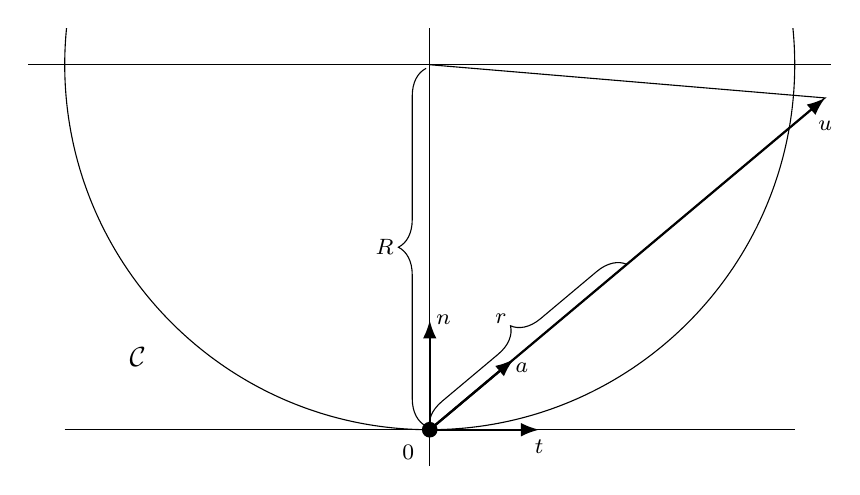
\begin{tikzpicture}
\begin{axis}[ 
    axis lines = middle,
    ticks = none,
    axis line style={-},
    ymin=-1.1, ymax=0.1,
    xmin=-1.1, xmax=1.1,
    axis equal image,
    height=4in
]

%\draw[color=white, fill = blue, opacity=0.2] (axis cs:-1.1, -1) rectangle (axis cs:1.1, 1.1);
%\draw[color=white, fill = gray, opacity=0.4] (axis cs:-1.1, -1.3) rectangle (axis cs:1.1, -1);

\def\figphi{10}
%p/4-phi/2=theta where phi is angle from x-axis of unit circle to top right point of triangle
\def\figtheta{45-\figphi/2}

\draw[color=black] (axis cs:-1, -1) -- (axis cs:1, -1);
  \node at (axis cs:-0.8, -0.8) {$\C$};
%\addplot[data cs=polar, red, opacity=0.6, domain=0:180,samples=180,smooth, fill=red, fill opacity=0.6, shift={(0, transformdirectiony(-1))}] (x, {cos(90 - x)});
\begin{scope}[shift={(0, transformdirectiony(-1))}]
  \node[label={225:{\footnotesize $0$}},circle,fill,inner sep=2pt] at (axis cs:0,0) {};
  %\draw (axis cs:0.25,0) arc(0:{\figtheta}:{transformdirectionx(0.25)});
  %\node at (axis cs:{0.17*cos(0.5*\figtheta)}, {0.17*sin(0.5*\figtheta)}) {$\theta$};
  \draw (axis cs:0,0) -- (axis cs:{1.1*2*sin(\figtheta)*cos(\figtheta)},{1.1*2*sin(\figtheta)*sin(\figtheta)}) -- (axis cs:0, 1);
  \draw [decorate,decoration={brace,amplitude=10pt}] (axis cs:0,0) -- (axis cs:{(1.1/2)*2*sin(\figtheta)*cos(\figtheta)},{(1.1/2)*2*sin(\figtheta)*sin(\figtheta)}) node [black,midway,yshift={transformdirectiony(0.1)}, xshift={transformdirectionx(-0.1)}] {\footnotesize $r$};
  %\draw [decorate,decoration={brace,amplitude=15pt, mirror}] (axis cs:0,0) -- (axis cs:{(1.1)*2*sin(\figtheta)*cos(\figtheta)},{(1.1)*2*sin(\figtheta)*sin(\figtheta)}) node [black,midway,yshift={transformdirectiony(-0.15)}, xshift={transformdirectionx(0.15)}] {\footnotesize $u$};
  \draw [-Latex,thick] (axis cs:0,0) -- (axis cs:{(1.1)*2*sin(\figtheta)*cos(\figtheta)},{(1.1)*2*sin(\figtheta)*sin(\figtheta)}) node [black,yshift={transformdirectiony(-0.1)}, xshift={transformdirectionx(0)}] {\footnotesize $u$};
\end{scope}


\draw [decorate,decoration={brace,amplitude=10pt,mirror}] (axis cs:-0.01,-0.01) -- (axis cs:-0.01,{-1+0.01}) node [black,midway,xshift={transformdirectionx(-0.15)}] {\footnotesize $R$};

%\draw [decorate,decoration={brace,amplitude=5pt}] (axis cs:0,-1) -- (axis cs:{0.5*cos(\figphi)},{0.5*(-sin(\figphi)-1)}) node [black,midway, xshift={transformdirectionx(-0.07)}, yshift={transformdirectiony(0.07)}] {\footnotesize $l$};

\draw [-Latex, thick] (axis cs:0,-1) -- (axis cs:{0.3*cos(\figtheta)},{0.3*sin(\figtheta)-1}) node [black, xshift={transformdirectionx(0.03)}, yshift={transformdirectiony(-0.03)}] {\footnotesize $a$};
\draw [-Latex, thick] (axis cs:0, -1) -- (axis cs:0.3, -1) node [black,xshift={transformdirectionx(0)},yshift={transformdirectiony(-0.06)}] {\footnotesize $t$};
\draw [-Latex, thick] (axis cs:0, -1) -- (axis cs:0, -0.7) node [black,xshift={transformdirectionx(0.05)},yshift={transformdirectiony(0)}] {\footnotesize $n$};
\draw (axis cs:0,0) circle [radius=1];

  %\node[label={{$-1$}}] at (axis cs:-0.5,0.5) {};
  %\node[label={{$-1$}}] at (axis cs:-0.5,-1.2) {};
  %\node[label={{$+1$}}] at (axis cs:-0.3,-0.7) {};

\end{axis}
\end{tikzpicture}
\end{center}
%:

  For any $P$ on the circle the distance between $0$ and $P$ is $2R\sin\theta$ where $\theta$ is the angle between $\overrightarrow{0P}$ and $t$ (you can see this by e.g. bisecting the triangle formed by $0, P$ and the center of the circle). Consequently, we only have an odd number of intersections when $\pdot{a}{n} > 0$ and when $\abs{u} > 2R\sin\theta$, where $\theta$ is the angle between $u$ and $t$. Notably $\abs{u} = 2r$ and since $a$ is a unit vector we have
  $$
  \pdot{a}{n}^2 + \pdot{a}{t}^2 = 1, \, \pdot{a}{t} = \abs{a}\abs{t}\cos\theta = \cos\theta \implies \pdot{a}{n}^2 = 1 - \cos^2 \theta = \sin^2\theta \implies \pdot{a}{n} = \abs{\sin\theta}.
  $$
  Since $\pdot{a}{n} > 0$ for any $(a,b,r)$ giving odd intersections, we know $\theta \in [0, \pi]$ and thus $\sin\theta = \abs{\sin\theta}$, so $\abs{u} > 2R\sin\theta \iff r > R\pdot{a}{n}$. Finally putting all this together we can explicitly write
  \begin{equation}
  \chit{\Ae}{a, b, r} = \begin{cases}
    1 & \pdot{a}{n} > 0, \, r < R \pdot{a}{n}, \\
    1 & \pdot{a}{n} < 0, \\
    -1 & \textup{otherwise}
  \end{cases}.
  \end{equation} \label{eq:2:chit}
  \newpage
  The picture also gives us helps us characterize $b$ in terms of $a$. Since we only care about the $b$ such that $\pdot{b}{t} > 0$, $\pdot{a}{n} > 0 \implies b = a^\perp$, i.e. $b$ is $a$ rotated clockwise. Otherwise, $b$ is a counterclockwise rotation so that $b = -a^\perp$, thus
  \begin{equation}
    b = \sgn{\dot{a}{n}} a^\perp. \label{eq:2:ba}
  \end{equation}

  We're able to use \eqref{eq:2:chit}, \eqref{eq:2:ba} to simplify our integrand i.e.
  \begin{IEEEeqnarray*}{rCl}
    \dot{\ks}{n} &=& \int_{\A} \chit{\Ae}{a, b, r} \sgn{\dot{a}{n}} \frac{\pdot{a}{t}\pdot{a^\perp}{n} - \pdot{a^\perp}{t}\pdot{a}{n}}{r^{1+\sigma}} \, d\haus{2}{a,b,r} \\
    &=& \int_{\A} \chit{\Ae}{a, b, r} \sgn{\dot{a}{n}} \frac{-\pdot{a}{t}\pdot{a}{t} - \pdot{a}{n}\pdot{a}{n}}{r^{1+\sigma}} \, d\haus{2}{a,b,r} \\
    &=& -\int_{\A} \frac{\chit{\Ae}{a, b, r} \sgn{\dot{a}{n}}}{r^{1+\sigma}} \, d\haus{2}{a,b,r}.
  \end{IEEEeqnarray*}

  Now, motivated by the picture above we do a change of variables $u := \phi(a,b,r) = 2ra$. We have
  $$
  \nabla \phi (a, b, r) =
  \begin{blockarray}{ccc}
    \frac{1}{\sqrt{2}}(b, -a, 0) & (0, 0, 1) \\
    \begin{block}{(cc)c}
      \sqrt{2}r\pdot{b}{t} & 2\pdot{a}{t} & t \\
      \sqrt{2}r\pdot{b}{n} & 2\pdot{a}{n} & n \\
    \end{block}
  \end{blockarray}
  $$
  so
  \begin{IEEEeqnarray*}{rCl}
    \parens{\JJ{\phi}(a,b,r)}^2 = \abs{\nabla \phi^T(a,b,r) \nabla\phi(a,b,r)} &=&
    \abs{\begin{pmatrix}
      \sqrt{2}r\pdot{b}{t} & \sqrt{2}r\pdot{b}{n} \\
      2\pdot{a}{t} & 2\pdot{a}{n}
    \end{pmatrix}
    \begin{pmatrix}
      \sqrt{2}r\pdot{b}{t} & 2\pdot{a}{t} \\
      \sqrt{2}r\pdot{b}{n} & 2\pdot{a}{n}
    \end{pmatrix}} \\
    &=&
    \abs{\begin{pmatrix}
      2r^2 & 2\sqrt{2}r \parens{\pdot{b}{t}\pdot{a}{t} + \pdot{b}{n}\pdot{a}{n}} \\
      2\sqrt{2}r \parens{\pdot{b}{t}\pdot{a}{t} + \pdot{b}{n}\pdot{a}{n}} & 4 \\
    \end{pmatrix}} \\
    &=& 8r^2 - 8\parens{\pdot{a}{t}}^2\pdot{b}{t}^2 + \pdot{a}{n}^2\pdot{b}{n}^2 + 2\pdot{a}{n}\pdot{a}{t}\pdot{b}{n}\pdot{b}{t} \\
    &=& 8r^2 - 8\parens{\pdot{a}{t}^2\pdot{a}{n}^2 + \pdot{a}{n}^2\pdot{a}{t}^2 - 2\pdot{a}{n}^2\pdot{a}{t}^2} \\
    \implies \JJ{\phi} &=& 2\sqrt{2}r.
  \end{IEEEeqnarray*}
  Combining this with the fact that
  $$
  \phi\parens{\A} = \R{2}, \,
  \phi^{-1}(u) = \parens{\frac{u}{\abs{u}}, \sgn{\dot{u}{n}} \frac{u^\perp}{\abs{u}}, \frac{\abs{u}}{2}},
  $$
  we now have
  $$
    \dot{\ks}{n} =
    -\int_{\R{2}}
    \frac{\chit{\Ae}{\frac{u}{\abs{u}}, \sgn{\dot{u}{n}} \frac{u^\perp}{\abs{u}}, \frac{\abs{u}}{2}}\sgn{\dot{u}{n}}}{\parens{\frac{\abs{u}}{2}}^{1+\sigma}} \frac{1}{\sqrt{2}\abs{u}}
    \, d\haus{2}{u}.
  $$
  To further simplify, put $\Pu := \braces{u \in \R{2} \mid \pdot{u}{n} < 0 \textup{ or } \frac{\abs{u}}{2} < R\pdot{\frac{u}{\abs{u}}}{n}}$ and notice
  $$
  \chit{\Ae}{\frac{u}{\abs{u}}, \sgn{\dot{u}{n}} \frac{u^\perp}{\abs{u}}} =
  \begin{cases}
    1 & \pdot{u}{n} > 0, \, \frac{\abs{u}}{2} < R \pdot{\frac{u}{\abs{u}}}{n}, \\
    1 & \pdot{u}{n} < 0, \\
    -1 & \textup{otherwise}
  \end{cases} = \chit{\Pu}{u}.
  $$
  So, further simplifying and leveraging \ref{lem:pu} we have
  $$
  \dot{\ks}{n} = -2^{\sigma+1/2}\int_{\R{2}} \frac{\chit{\Pu}{u}\sgn{\dot{u}{n}}}{\abs{u}^{2+\sigma}} \, d\haus{2}{u} = -2^{\sigma+1/2} \frac{-2^{1-\sigma}}{\sigma R^{\sigma}} \B{\frac{1}{2},\frac{1-\sigma}{2}} = \frac{2^{3/2}}{\sigma R^\sigma} \B{\frac{1}{2}, \frac{1-\sigma}{2}}.
  $$

\end{proof}
%:

\section{Non-local Curvature of a Circle in N-D}%;
\begin{theorem}
  For a circle of radius $R$ in $\R{n}$
  $$
    \ks(z) = \frac{2^{1/2} \pi^{n-1}}{\sigma R^\sigma} \frac{\G{1+\sigma/2} \G{(1-\sigma)/2}}{\G{(n+1)/2}\G{(n+\sigma)/2}\G{1-\sigma/2}} n(z)
  $$
\end{theorem}
\begin{proof}
  Our strategy for this proof is as follows
  \begin{itemize}
    \item[\ref{nd:sect:2d}] Recognize the similarity with the 2D case and slice the domain along each $u$ in \eqref{lem:pu}.
    \item[\ref{nd:sect:norm}] Show $\ks \cdot m = 0 \, \forall m \in \{n\}^\perp$ so that we can focus on $\ks \cdot n$.
    \item[\ref{nd:sect:radii}] Slice along each radius $r$ to further simplify the computation.
    \item[\ref{nd:sect:sphere}] Show the domain of the inner-most integral with $u, r$ fixed is a pair of spheres.
    \item[\ref{nd:sect:eval}] Evaluate the final integrals.
  \end{itemize}

  \noindent As with the 2D case, due to symmetry we know $\ks(z) = \ks$, and
  \begin{IEEEeqnarray}{ll}
    \frac{\omega_{n-3}^2}{\sigma R^\sigma \sqrt{2}} &\B{\frac{3}{2}, \frac{n-2}{2}} \B{\frac{\sigma+2}{2}, \frac{n-2}{2}} \B{\frac{1}{2}, \frac{1-\sigma}{2}} \label{nd:eq:0} \\
    &= \frac{1}{\sigma R^\sigma \sqrt{2}} \parens{\frac{2\pi^{n/2 -1}}{\G{n/2-1}}}^2 \frac{\G{3/2}\G{n/2-1}}{\G{(n+1)/2}} \frac{\G{\sigma/2+1}\G{n/2-1}}{\G{(n+\sigma)/2}} \frac{\G{1/2}\G{(1-\sigma)/2}}{\G{1-\sigma/2}} \nonumber \\
    &= \frac{2^{3/2} \pi^{n-2}}{\sigma R^\sigma} \frac{\G{3/2}\G{1/2}\G{1+\sigma/2} \G{(1-\sigma)/2}}{\G{(n+1)/2}\G{(n+\sigma)/2}\G{1-\sigma/2}} \nonumber \\
    &= \frac{2^{1/2} \pi^{n-1}}{\sigma R^\sigma} \frac{\G{1+\sigma/2} \G{(1-\sigma)/2}}{\G{(n+1)/2}\G{(n+\sigma)/2}\G{1-\sigma/2}}, \nonumber
  \end{IEEEeqnarray}
  so that our task is to show
  $$
  \ks = \frac{\omega_{n-3}^2}{\sigma R^\sigma \sqrt{2}} \B{\frac{3}{2}, \frac{n-2}{2}} \B{\frac{\sigma+2}{2}, \frac{n-2}{2}} \B{\frac{1}{2}, \frac{1-\sigma}{2}} n(z).
  $$
  \subsection{Similarity to 2D} \label{nd:sect:2d}%;
  Since $\C \subset \lsp{t, n}$, we can simplify our calculation by slicing at each $u \in \R{2}$ representing $\D{ra, b, r} \cap \S$. To that end, put $\Psi : \mathcal{A}^+ \to \mathbb{R}^2$  so that
  $$
  \D{ra, b, r} \cap S = \braces{ t \Psi(a, b, r) \mid t \in [0, 1] }.
  $$
  In order to to determine an exact formula for $\Psi$, note the following, where $u := \Psi(a, b, r)$:
\begin{itemize}
  \item There is an isoceles triangle formed by the center of $\D{ra, b, r}$ and the endpoints of $\D{ra, b, r} \cap S$, and thus the component of $ra$ in the direction of $u$ must be half of $u$'s length, i.e.
    \begin{equation}
      \dot{ra}{\frac{u}{\abs{u}}} = \frac{\abs{u}}{2} \implies 2 \pdot{ra}{u} = \abs{u}^2 = \dot{u}{u}, \label{nd:c1}
    \end{equation}
  \item Since $\D{ra, b, r} \cap \S \subset \D{ra, b, r}, \, \forall x \in \D{ra, b, r} \cap \S$
    \begin{equation}
      \dot{b}{x} = 0 \implies \dot{b}{u} = 0. \label{nd:c2}
    \end{equation}
\end{itemize}
  Since $u \in \S$, we can expand via the $\braces{t, n}$ basis, take into account \eqref{nd:c2}, and the fact that $\dot{b}{t} > 0$ to see
\begin{equation}
  0 = \dot{b}{u} = b_tu_t + b_nu_n \implies u_t = \frac{-b_n u_n}{b_t}. \label{nd:e1}
\end{equation}

Substituting this back into \eqref{nd:c1} we have
\begin{IEEEeqnarray*}{rCl}
  2ra_nu_n - 2r a_t \frac{b_n u_n}{b_t} = u_n^2 + \frac{b_n^2 u_n^2}{b_t^2} &\implies& u_n^2 \parens{1 + \frac{b_n^2}{b_t^2}} + 2r u_n \parens{\frac{a_t b_n}{b_t} - a_n} = 0\\
  &\implies& u_n = 0 \lor u_n \frac{b_t^2 + b_n^2}{b_t^2} + 2r \frac{a_t b_n - a_n b_t}{b_t} = 0.
\end{IEEEeqnarray*}
Notably $u_n \neq 0$ since otherwise \eqref{nd:e1} would force $u_t = 0$, i.e. $u = 0$, which only occurs for a measure-zero set of $(a, b, r) \in \A$. Solving the above equation for $u_n$ we find
$$
  u_n = -2r\frac{a_t b_n - a_n b_t}{b_t} \frac{b_t^2}{b_t^2 + b_n^2} = 2r \frac{a_n b_t - a_t b_n}{b_t^2 + b_n^2} b_t.
$$
  Putting $\Prs := \parens{t \otimes t} + \parens{n \otimes n}$ and plugging this back into \eqref{nd:e1} we find
$$
  \Psi(a, b, r) = 2r \frac{a_n b_t - a_t b_n}{\Prsbpa^2} \parens{b_t n - b_n t} = 2r \frac{a_t b_n - a_n b_t}{\Prsbpa^2} \Prsbp
$$
  We can further rewrite this by noticing
$$
  \dot{\Prsbp}{a} = \dot{\parens{b_t t + b_n n}^\perp}{a} = \dot{\parens{b_n t - b_t n}}{a} = b_n a_t - b_t a_n,
$$
  and putting
  \begin{equation}
  p(b) = \frac{\Prsbp}{\Prsbpa}, \label{nd:def:p}
  \end{equation}
  so that
\begin{equation}
  \Psi(a, b, r) = 2r \frac{\dot{\Prsbp}{a}}{\Prsbpa^2} \mathcal{P}_S b^\perp = 2r \pdot{p(b)}{a} p(b) = 2r \parens{p(b) \otimes p(b)}a. \label{nd:def:psi}
\end{equation}

Put $\E{u} := \Psi^{-1}(\braces{u})$, with \ref{lem:co:psi} we see
$$
  \ks
  = \frac{1}{\sqrt{2}} \int_{\mathbb{R}^2} \frac{1}{\abs{u}} \int_{\E{u}}
  \chit{\A}{a,b,r} \frac{\pdot{a}{t}b - \pdot{b}{t}a}{r^{1+\sigma}}
  \frac{\Prsbpa}{\sqrt{2 - \frac{\abs{u}^2}{4r^2}} \sqrt{r^2 - \parens{r^2-1} \frac{\abs{u}^2}{4r^2} }}
  \, d\haus{2n-4}{a, b, r} \, d\haus{2}{u}.
$$
As noticed above $\C \in \S$ so $\chit{\A}{a,b,r}$ must only depend on where $\D{a,b,r} \cap \S$, i.e. $u$. Putting
$$\Pu := \braces{ u \in \S \mid \pdot{u}{n} < 0 \textup{ or } \frac{\abs{u}}{2} < R\parens{\frac{u}{\abs{u}} \cdot n} }$$
we must have $\chit{\A}{a,b,r} = \chit{\Pu}{u}$\footnote{$\Pu$ is notably the same as in the 2D case. This comes from the inherent geometry of the circle, i.e. this set includes all $u$ who point below the circle (i.e. $\pdot{u}{n} < 0$), or $u$ that lie within the interior of the circle, i.e. $\abs{u} < 2R\sin\theta$ where $\theta$ is the angle between $t$ and $u$.}, and so
\begin{equation}
  \ks
  = \frac{1}{\sqrt{2}} \int_{\mathbb{R}^2} \frac{\chit{\Pu}{u}}{\abs{u}} \int_{\E{u}}
  \frac{\pdot{a}{t}b - \pdot{b}{t}a}{r^{1+\sigma}}
  \frac{\Prsbpa}{\sqrt{2 - \frac{\abs{u}^2}{4r^2}} \sqrt{r^2 - \parens{r^2-1} \frac{\abs{u}^2}{4r^2} }}
  \, d\haus{2n-4}{a, b, r} \, d\haus{2}{u}. \label{nd:eq:1}
\end{equation}%:
\subsection{Normal Component Projection} \label{nd:sect:norm}%;
  We want to show $\ks = \parens{n \otimes n}\ks$. Just as with the 2D case it's trivial to see $\pdot{\ks}{t} = 0$. In order to show $\pdot{\ks}{m} = 0$ for $m \in \U{\braces{n,t}^\perp}$, we'll show that the integrand of \eqref{nd:eq:1} dotted with $m$
  \begin{equation}
    \frac{\chit{\Pu}{u}}{\abs{u}} \frac{\pdot{a}{t}\pdot{b}{m} - \pdot{b}{t}\pdot{a}{m}}{r^{1+\sigma}} \frac{\Prsbpa}{\sqrt{2 - \frac{\abs{u}^2}{4r^2}} \sqrt{r^2 - \parens{r^2-1} \frac{\abs{u}^2}{4r^2} }}, \label{nd:eq:normintegrand}
  \end{equation}
  is odd over a symmetric domain.

  Specifically, we hope to show, for $R_m := I - 2(m \otimes m)$, $(u, a, b, r) \to (u, R_m a, R_m b, r)$ is an isomorphism that the integrand is odd under. From \eqref{nd:def:p} $p(R_m b) = p(b)$ and thus \eqref{nd:def:psi} says
  $$
  \Psi(R_m a, R_m b, r) = 2r \pdot{p(R_m b)}{R_m a}p(R_m b) = 2r \pdot{p(b)}{R_m a}p(b) = 2r \pdot{p(b)}{a} p(b) = \Psi(a, b, r).
  $$
  This tells us that $u$ is invariant under $(a, b) \to (R_m a, R_m b)$ transformation. By a similar observation $\Prsbpa$ is invariant under a $b \to R_m b$ transformation, and thus the task of showing \eqref{nd:eq:normintegrand} is odd under $(u, a, b, r) \to (u, R_m a, R_m b, r)$ reduces to showing
  $$
  J(a, b) := \pdot{a}{t}\pdot{b}{m} - \pdot{b}{t}\pdot{a}{m}
  $$
  is odd under the $(a, b) \to (R_m a, R_m b)$ transformation. Indeed we can see
  \begin{IEEEeqnarray*}{rCl}
    J( R_m a, R_m b) &=& \pdot{R_m a}{t}\pdot{R_m b}{m} - \pdot{R_m b}{t}\pdot{R_m a}{m} \\
    &=& \pdot{\parens{a - 2\pdot{a}{m}m}}{t}\pdot{\parens{b - 2\pdot{b}{m}m}}{m} - \pdot{\parens{b - 2\pdot{b}{m}m}}{t}\pdot{\parens{a - 2\pdot{a}{m}m}}{m} \\
    &=& \parens{\pdot{a}{t} - 2\pdot{a}{m}\pdot{m}{t}}\parens{\pdot{b}{m} - 2\pdot{b}{m}} - \parens{\pdot{b}{t} - 2\pdot{b}{m}\pdot{m}{t}}\parens{\pdot{a}{m} - 2\pdot{a}{m}} \\
    &=& \parens{\pdot{a}{t} - 0}\parens{-\pdot{b}{m}} - \parens{\pdot{b}{t} - 0}\parens{-\pdot{a}{m}} \\
    &=& -\pdot{a}{t}\pdot{b}{m} + \pdot{b}{t}\pdot{a}{m} = - J(a, b, r).
  \end{IEEEeqnarray*}
  Lastly due to the invariance of $u$, the fact that $R_m$ is an isomorphism, $\pdot{R_m b}{t} = \pdot{b}{t}$ and
  $$
  \pdot{R_m a}{R_m b} = \pdot{\parens{a - 2\pdot{m}{a}m}}{\parens{b - 2\pdot{m}{b}m}} = \pdot{a}{b}
  $$
  we have $(a, b, r) \in \E{u} \iff (R_m a, R_m b, r) \in \E{u}$. Thus, for the rest of the proof we may focus on $\dot{\ks}{n}$. Before expanding our integral, notice
  $$
  \pdot{a}{t}\pdot{b}{n} - \pdot{b}{t}\pdot{a}{n} = \dot{\parens{\pdot{b}{n}t - \pdot{b}{t}n}}{a} = \dot{- \Prsbp}{a}
  $$
  and since $u = \frac{2r}{\Prsbpa^2} \pdot{\Prsbp}{a} \Prsbp \implies \abs{\dot{\Prsbp}{a}} = \frac{\abs{u}\Prsbpa}{2r}$, $\sgn{\dot{\Prsbp}{a}} = \sgn{\dot{\Prsbp}{u}}$ we have
  \begin{equation}
    \dot{\ks}{n}
    = \frac{-1}{2\sqrt{2}} \int_{\mathbb{R}^2} \chit{\Pu}{u} \int_{\E{u}}
    \frac{1}{r^{2+\sigma}}
    \frac{\sgn{\dot{\Prsbp}{u}} \Prsbpa^2}{\sqrt{2 - \frac{\abs{u}^2}{4r^2}} \sqrt{r^2 - \parens{r^2-1} \frac{\abs{u}^2}{4r^2} }}
    \, d\haus{2n-4}{a, b, r} \, d\haus{2}{u}. \label{nd:eq:2}
  \end{equation}
  %:
\subsection{Slicing Along Radii} \label{nd:sect:radii}%;
Next, to further simplify \eqref{nd:eq:2}, let's slice along each $r$, i.e. put $\Phi : \E{u} \to \R{+}$ given by
\begin{equation}
  \Phi(a, b, r) = r. \label{nd:def:phi}
\end{equation}

Put $\E{u, r} = \Phi^{-1}(\{r\})$, so that with the co-area calculation in \ref{lem:co:phi} we find \eqref{nd:eq:2} becomes
\begin{IEEEeqnarray}{ll}
  \frac{-1}{2\sqrt{2}} &\int_{\mathbb{R}^2} \chit{\Pu}{u} \int_{\E{u}}
  \frac{1}{r^{2+\sigma}}
  \frac{\sgn{\dot{\Prsbp}{u}} \Prsbpa^2}{\sqrt{2 - \frac{\abs{u}^2}{4r^2}} \sqrt{r^2 - \parens{r^2-1} \frac{\abs{u}^2}{4r^2} }}
  \, d\haus{2n-4}{a, b, r} \, d\haus{2}{u} \nonumber \\
  &=
  \frac{-1}{2\sqrt{2}} \int_{\mathbb{R}^2} \chit{\Pu}{u} \int_{\Phi(\E{u})} \int_{\E{u, r}}
  \frac{1}{r^{3+\sigma}}
  \frac{\sgn{\dot{\Prsbp}{u}} \Prsbpa^2}{\sqrt{2 - \frac{\abs{u}^2}{4r^2}} \sqrt{1-\frac{\abs{u}^2}{4r^2}}}
  \, d\haus{2n-5}{a, b} \, dr \, d\haus{2}{u} \nonumber \\
  &=
  \frac{-1}{2\sqrt{2}}
  \int_{\mathbb{R}^2} \chit{\Pu}{u}
  \int_{\Phi(\E{u})} \frac{1}{r^{3+\sigma} \sqrt{2 - \frac{\abs{u}^2}{4r^2}} \sqrt{1-\frac{\abs{u}^2}{4r^2}}}
  \int_{\E{u, r}} \sgn{\dot{\Prsbp}{u}} \Prsbpa^2
  \, d\haus{2n-5}{a, b} \, dr \, d\haus{2}{u} \nonumber \\ & \label{nd:eq:3}
\end{IEEEeqnarray}
%:
\subsection{Splitting Spheres} \label{nd:sect:sphere} %;
Since the inner most integrand in \eqref{nd:eq:3} only depends on $b$, and by the uniform nature of
$$
\E{u, r} = \braces{ (a, b) \in \UTP{} \mid \dot{b}{t} > 0, \, \dot{u}{b} = 0 \textup{ and } 2r\pdot{u}{a} = \pdot{u}{u} },
$$
it's natural to slice on each $b$, so put $\Xi : \E{u, r} \to \Et{u, r}$ where $\Xi(a, b) = b$. With the calculation done in \ref{lem:co:xi} we can see, after putting $\E{u, r, b} = \Xi^{-1}(b)$ and including \ref{lem:co:xi}, \ref{lem:measure:eurb}, \eqref{nd:eq:3} becomes
\begin{IEEEeqnarray}{ll}
  &\frac{-1}{2\sqrt{2}}
  \int_{\mathbb{R}^2} \chit{\Pu}{u}
  \int_{\Phi(\E{u})} \frac{}{r^{3+\sigma} \sqrt{2 - \frac{\abs{u}^2}{4r^2}} \sqrt{1-\frac{\abs{u}^2}{4r^2}}}
  \int_{\Et{u, r}} \sgn{\dot{\Prsbp}{u}} \Prsbpa^2
  \frac{\haus{n-3}{\E{u, r, b}}}{\parens{2 - \frac{\abs{u}^2}{4r^2}}^{-1/2}}
  \, d\haus{n-2}{b} \, dr \, d\haus{2}{u} \nonumber \\
  &=
  \frac{-\omega_{n-3}}{2\sqrt{2}}
  \int_{\mathbb{R}^2} \chit{\Pu}{u}
  \int_{\Phi(\E{u})} \frac{\parens{1-\frac{\abs{u}^2}{4r^2}}^{(n-4)/2}}{r^{3+\sigma}}
  \int_{\Et{u, r}} \sgn{\dot{\Prsbp}{u}} \Prsbpa^2
  \, d\haus{n-2}{b} \, dr \, d\haus{2}{u} \label{nd:eq:5}
\end{IEEEeqnarray}
To evaluate this second integral we'll need one more application of the co-area formula; we'll split using
$$
\zeta : \Et{u, r} \to [-1, 1] \textup{ given by } \zeta(b) = \dot{b}{\frac{u^\perp}{\abs{u^\perp}}}.
$$
This is a natural transformation since
\begin{equation}
\Prsbp = \parens{\pdot{b}{\frac{u}{\abs{u}}} \frac{u}{\abs{u}} + \pdot{b}{\frac{u^\perp}{\abs{u^\perp}}} \frac{u^\perp}{\abs{u^\perp}}}^\perp = -\pdot{b}{\frac{u^\perp}{\abs{u^\perp}}} \frac{u}{\abs{u^\perp}}
  = -\zeta(b) \frac{u}{\abs{u^\perp}} \label{nd:eq:6}
\end{equation}
Further, since $\R{n} = \lsp{ \frac{u}{\abs{u}}, \frac{u^\perp}{\abs{u^\perp}}, f_1, f_2, \ldots f_{n-2} }$ for some orthonormal $f_i$, it's true that
$$
\zeta(b)^2 + \pdot{b}{f_1}^2 + \pdot{b}{f_2}^2 + \cdots + \pdot{b}{f_{n-2}}^2 = 1 \implies \pdot{b}{f_1}^2 + \pdot{b}{f_2}^2 + \cdots + \pdot{b}{f_{n-2}}^2 = 1 - \zeta(b)^2,
$$
and so
\begin{IEEEeqnarray}{rCl}
  \zeta^{-1}(v) &=& \braces{ b \in \U{\braces{u}^\perp} \mid v = \pdot{b}{\frac{u^\perp}{\abs{u^\perp}}} } \nonumber \\
  &=& \braces{ b \in \U{\braces{u}^\perp} \mid \pdot{b}{f_1}^2 + \pdot{b}{f_2}^2 + \cdots + \pdot{b}{f_{n-2}}^2 = 1 - v^2 } \nonumber \\
  &=& S_{n-3}\parens{\sqrt{1-v^2}} \label{nd:eq:7}
\end{IEEEeqnarray}
Combining \eqref{nd:eq:6}, \eqref{nd:eq:7} and \ref{lem:co:zeta}, the inner most integral of \eqref{nd:eq:5} becomes
\begin{IEEEeqnarray}{rCl}
  \int_{\Et{u, r}} \sgn{\dot{\Prsbp}{u}} \Prsbpa^2 \, d\haus{n-2}{b} &=& \int_{\zeta\parens{\Et{u,r}}} \sgn{\dot{-v \frac{u}{\abs{u^\perp}}}{u}} v^2 \, \frac{\haus{n-3}{\zeta^{-1}(v)}}{\sqrt{1-v^2}} \, dv \nonumber \\
  &=& - \omega_{n-3} \int_{\zeta\parens{\Et{u, r}}} \sgn{v} v^2 \parens{1 - v^2}^{(n-4)/2} \, dv. \label{nd:eq:8}
\end{IEEEeqnarray}
To better understand $\zeta\parens{\Et{u,r}}$ notice $b \in \Et{u, r} \implies \dot{b}{t} > 0$, so
$$
0 < b \cdot t = \parens{b \cdot \frac{u}{\abs{u}}} \parens{t \cdot \frac{u}{\abs{u}}} + \parens{b \cdot \frac{u^\perp}{\abs{u^\perp}}} \parens{t \cdot \frac{u^\perp}{\abs{u^\perp}}} = \parens{b \cdot \frac{u^\perp}{\abs{u^\perp}}} \parens{t \cdot \frac{u^\perp}{\abs{u^\perp}}},
$$
i.e. $\zeta\parens{\Et{u, r}} = [-1, 0]$ if $\sgn{\dot{t}{u^\perp}} = -1$ and $[0, 1]$ otherwise. Since the integrand in \eqref{nd:eq:8} is odd, we can integrate over $[0, 1]$ and multiply by $\sgn{\dot{t}{u^\perp}}$ to take this into account. As we expand \eqref{nd:eq:8}, note $\sgn{\dot{t}{u^\perp}} = -\sgn{\dot{n}{u}}$, so that
\begin{IEEEeqnarray}{rCl}
  \omega_{n-3} \int_{\zeta\parens{\Et{u, r}}} \sgn{v} v^2 \parens{1 - v^2}^{(n-4)/2} \, dv &=& \sgn{\dot{n}{u}} \omega_{n-3} \int_0^1 v^2 \parens{1-v^2}^{(n-4)/2} \, dv \nonumber \\
  &=& \frac{\sgn{\dot{n}{u}} \omega_{n-3}}{2} \int_0^1 v^{1/2} \parens{1 - v}^{(n-4)/2} \, dv \nonumber \\
  &=& \frac{\sgn{\dot{n}{u}} \omega_{n-3}}{2} \B{\frac{3}{2}, \frac{n-2}{2}} \label{nd:eq:9}
\end{IEEEeqnarray}

Putting \eqref{nd:eq:9} back into \eqref{nd:eq:5} our calculation becomes
\begin{equation}
  \dot{\ks}{n} = \frac{-\omega_{n-3}^2}{4\sqrt{2}} \B{\frac{3}{2}, \frac{n-2}{2}}
  \int_{\R{2}} \chit{\Pu}{u} \sgn{\dot{n}{u}}
  \int_{\Phi\parens{\E{u}}} \frac{\parens{1 - \frac{\abs{u}^2}{4r^2}}^{(n-4)/2}}{r^{3+\sigma}}
  \, dr \, d\haus{2}{u}.
  \label{nd:eq:10}
\end{equation}
%:
\subsection{Evaluating Integrals} \label{nd:sect:eval}%;
To evaluate the final integrals we recall $\E{u} = \Psi^{-1}\parens{\braces{u}}$ where $\Psi$ is given in \eqref{nd:def:psi}. By definition of $\Phi$ in \eqref{nd:def:phi} we have
$$
\Phi\parens{\E{u}} = \Phi\parens{\Psi^{-1}\parens{\braces{u}}} = \braces{ r \mid 2r \pdot{p(b)}{a} p(b) = u \textup{ for some } (a, b, r) \in \A} = \braces{r \mid r \ge \abs{u}{2} },
$$
so that the inner integral in \eqref{nd:eq:10}, after applying the transformation $r \to \frac{\abs{u}}{2} s^{-1/2}$, is
\begin{IEEEeqnarray}{rCl}
  \int_{\Phi\parens{\E{u}}} \frac{\parens{1 - \frac{\abs{u}^2}{4r^2}}^{(n-4)/2}}{r^{3+\sigma}} \,dr &=& \int_{\abs{u}/2}^\infty \parens{r^2 - \frac{\abs{u}^2}{4}}^{(n-4)/2} r^{1-\sigma-n} \, dr \nonumber \\
  &=& \int_1^0 \parens{\frac{\abs{u}^2}{4} \frac{1}{s} - \frac{\abs{u}^2}{4}}^{(n-4)/2} \parens{\frac{\abs{u}}{2}}^{1-\sigma-n} s^{(n+\sigma-1)/2} \frac{-\abs{u}}{4} s^{-3/2} \, ds \nonumber \\
  &=& \parens{\frac{\abs{u}}{2}}^{(n-4)+1-\sigma-n} \frac{\abs{u}}{4} \int_0^1 \parens{\frac{1 - s}{s}}^{(n-4)/2} s^{(n+\sigma-4)/2} \, ds \nonumber \\
  &=& \frac{\abs{u}^{-2-\sigma}}{2^{-1-\sigma}} \int_0^1 \parens{1-s}^{(n-4)/2} s^{\sigma/2} \, ds \nonumber \\
  &=& \frac{2^{1+\sigma}}{\abs{u}^{2+\sigma}} \B{\frac{\sigma+2}{2}, \frac{n-2}{2}}. \label{nd:eq:11}
\end{IEEEeqnarray}
Plugging \eqref{nd:eq:11} back into \eqref{nd:eq:10} our calculation simplifies to
\begin{IEEEeqnarray}{rCl}
  \dot{\ks}{n} &=& \frac{-\omega_{n-3}^2}{4\sqrt{2}} \B{\frac{3}{2}, \frac{n-2}{2}}
  \int_{\R{2}} \chit{\Pu}{u} \sgn{\dot{n}{u}}
  \int_{\Phi\parens{\E{u}}} \frac{\parens{1 - \frac{\abs{u}^2}{4r^2}}^{(n-4)/2}}{r^{3+\sigma}}
  \, dr \, d\haus{2}{u} \nonumber \\
  &=&
  -2^{1+\sigma-5/2}\omega_{n-3}^2 \B{\frac{3}{2}, \frac{n-2}{2}} \B{\frac{\sigma+2}{2}, \frac{n-2}{2}}
  \int_{\R{2}} \frac{\chit{\Pu}{u} \sgn{\dot{n}{u}}}{\abs{u}^{2+\sigma}} \, d\haus{2}{u} \nonumber \\
  &=& -2^{\sigma-3/2} \omega_{n-3}^2 \B{\frac{3}{2}, \frac{n-2}{2}} \B{\frac{\sigma+2}{2}, \frac{n-2}{2}} \frac{-2^{1-\sigma}}{\sigma R^\sigma} \B{\frac{1}{2}, \frac{1-\sigma}{2}} \label{nd:eq:12} \\
  &=& \frac{\omega_{n-3}^2}{\sigma R^\sigma\sqrt{2}} \B{\frac{3}{2}, \frac{n-2}{2}} \B{\frac{\sigma+2}{2}, \frac{n-2}{2}} \B{\frac{1}{2}, \frac{1-\sigma}{2}}, \label{nd:eq:13}
\end{IEEEeqnarray}
where in \eqref{nd:eq:12} we leveraged \ref{lem:pu}. Finally our desired equality follows after combining \eqref{nd:eq:13} with \eqref{nd:eq:0}.
%:
\end{proof}
%:

\section{Appendix}%;

\subsection{Supplementary Calculations}

\begin{lemma} \label{lem:pu}%;
\addcontentsline{toc}{subsubsection}{Fundamental 2D Integral}
  For $\Pu := \braces{u \in \R{2} \mid \pdot{u}{n} < 0 \textup{ or } \frac{\abs{u}}{2} < R\pdot{\frac{u}{\abs{u}}}{n}}$ we have
  $$
  \int_{\R{2}} \frac{\chit{\Pu}{u}\sgn{\dot{u}{n}}}{\abs{u}^{2+\sigma}} \, d\haus{2}{u} = \frac{-2^{1-\sigma}}{\sigma R^{\sigma}} \B{\frac{1}{2}, \frac{1-\sigma}{2}}
  $$
\end{lemma}
\begin{proof}
  Begin by putting
$$
I = \int_{\R{2}} \frac{\chit{\Pu}{u}\sgn{\dot{u}{n}}}{\abs{u}^{2+\sigma}} \, d\haus{2}{u}.
$$
Notably, this integral needs to be taken in a principal value sense, i.e.
$$
  I = \lim_{\epsilon \downarrow 0} \int_{\R{2} \setminus B_\epsilon} \frac{\chit{\Pu}{u}\sgn{\dot{u}{n}}}{\abs{u}^{2+\sigma}} \, d\haus{2}{u},
$$
where $B_\epsilon = \braces{ x \in \R{2} \mid \abs{x} = \epsilon }$. Next, substituting $u = r\cos\theta t + r\sin\theta n$ shows that
$$
  I = \lim_{\epsilon \downarrow 0} \int_0^{2\pi}\int_\epsilon^\infty \frac{\chit{\Pu}{r\cos\theta t + r\sin\theta n}\sgn{\sin\theta}}{r^{2+\sigma}} r \, dr \, d\theta,
$$
and further noting
\begin{IEEEeqnarray*}{rCl}
  \chit{\Pu}{r\cos\theta t + r\sin\theta n} &=& \begin{cases}
    1 & \theta \in [0, \pi], \frac{r}{2} < R\sin\theta \\
    1 & \theta \in [\pi, 2\pi] \\
    0 & \textup{otherwise}
  \end{cases} \\
  \sgn{\sin\theta} &=& \begin{cases} 1 & \theta \in [0, \pi] \\ -1 & \theta\in [\pi, 2\pi] \end{cases},
\end{IEEEeqnarray*}
means
\begin{IEEEeqnarray*}{rCl}
  I &=&
  \lim_{\epsilon \downarrow 0}
  \int_0^{\pi} \parens{
    \int_\epsilon^{2 R\sin\theta} \frac{1 \cdot 1}{r^{1+\sigma}} \, dr
    + \int_{2 R \sin\theta}^\infty \frac{-1 \cdot 1}{r^{1+\sigma}} \, dr
  } + \int_\pi^{2\pi} \parens{
    \int_\epsilon^\infty \frac{1 \cdot \parens{-1}}{r^{1+\sigma}} \, dr
  }
  \, d\theta \\
  &=& \lim_{\epsilon \downarrow 0}
  \frac{1}{-\sigma} \int_0^\pi \parens{ \left. r^{-\sigma}\right|_\epsilon^{2 R \sin\theta} - \left. r^{-\sigma}\right|_{2 R \sin\theta}^{\infty} } \, d\theta
  - \frac{1}{-\sigma} \int_\pi^{2\pi} \left. r^{-\sigma}\right|_{\epsilon}^\infty \, d\theta \\
  &=& \frac{-1}{\sigma} \lim_{\epsilon \downarrow 0} \int_0^\pi \parens{2 R\sin\theta}^{-\sigma} - \epsilon^{-\sigma} + \parens{2 R\sin\theta}^{-\sigma} \, d\theta
  + \int_\pi^{2\pi} \epsilon^{-\sigma} \, d\theta \\
  &=& \frac{-1}{\sigma} \lim_{\epsilon \downarrow 0} 2\int_0^\pi \parens{2R\sin \theta}^{-\sigma} \, d\theta -\pi \epsilon^{-\sigma} + \pi \epsilon^{-\sigma} \\
  &=& \frac{-2^{1-\sigma}}{\sigma R^\sigma} \int_0^\pi \parens{\sin\theta}^{-\sigma} \, d\theta \\
  &=& \frac{-2^{1-\sigma}}{\sigma R^\sigma} \int_{\pi / 2}^{-\pi/2} \parens{\cos\theta}^{-\sigma} \, \parens{- d\theta} \textup{ via } \theta \to \frac{\pi}{2} - \theta \\
  &=& \frac{-2^{1-\sigma}}{\sigma R^\sigma} 2\int_0^{\pi / 2} \parens{\cos\theta}^{-\sigma} \, d\theta = \frac{-2^{1-\sigma}}{\sigma R^\sigma} \B{\frac{1}{2}, \frac{1-\sigma}{2}}
\end{IEEEeqnarray*}
\end{proof}%:

\begin{lemma} \label{lem:co:psi}%;
\addcontentsline{toc}{subsubsection}{\texorpdfstring{$\Psi$ Co-Area Jacobian}{Ψ Co-Area Jacobian}}
  For $\Psi : \A \to \R{2}$ given by $\Psi(a, b, r) = 2r\parens{p(b) \otimes p(b)}a$, where $p(b) = \frac{\Prsbp}{\Prsbpa}$
  $$
  \J{\Psi}(a, b, r) = \frac{\sqrt{2}\abs{u}}{\Prsbpa} \sqrt{2 - \frac{\abs{u}^2}{4r^2}} \sqrt{r^2 - \parens{r^2-1} \frac{\abs{u}^2}{4r^2} }.
  $$
\end{lemma}
\begin{proof}
  Put $c = \frac{u - \pdot{u}{a}a}{\sqrt{\pdot{u}{u} - \pdot{u}{a}}}$ and $\braces{e_i}_{i=1}^{n-3}$ so that $\braces{a, b, c, e_1, ..., e_{n-3}}$ is an orthonormal basis spanning $\R{n}$.  We can use this basis to characterize
$$
  \T{\A}{(a, b, r)} = \lsp{ (e_i, 0, 0), (0, e_i, 0), (c, 0, 0), (0, c, 0), \eab, (0, 0, 1) \mid i = 1, ... (n-3)},
$$
  where $\eab := \frac{1}{\sqrt{2}} (b, -a, 0)$. Additionally, we can use the fact that $p(b), p(b)^\perp$ are an orthonormal basis spanning $\S$ to see $\T{\S}{\Psi(a, b, r)} = \lsp{p(b), p(b)^\perp}$. Next, we compute derivatives along flows as follows:
  \begin{IEEEeqnarray*}{rCl}
    \flowder{\Psi}{(e_i, 0, 0)} &=& 2r \parens{p(b) \otimes p(b)} e_i = 2r \pdot{p(b)}{e_i} p(b) = 0, \\
    \flowder{\Psi}{(c, 0, 0)} &=& 2r \parens{p(b) \otimes p(b)} c = 2r \pdot{p(b)}{c} p(b), \\
    \flowder{\Psi}{(0, 0, 1)} &=& 2 \pdot{p(b)}{a}p(b).
  \end{IEEEeqnarray*}
  For our last calculations we'll need the following, for $\beta : \R{1} \to \U{}$ such that $\beta(0) = b$:
\begin{IEEEeqnarray}{rCl}
  \left. \dby{s} p(\beta(s)) \right|_{s=0} &=& \frac{\Prs \beta '(0)^\perp}{\Prsbpa} - \frac{1}{\Prsbpa^3} \Prsbp \otimes \parens{\Prs \beta '(0)^\perp}^T \Prsbp = \frac{1}{\Prsbpa} \parens{1 - \parens{p(b) \otimes p(b)}} \Prs \beta '(0)^\perp \nonumber \\
  &=& \frac{1}{\Prsbpa} \parens{p(b) \otimes p(b) + p(b)^\perp \otimes p(b)^\perp - p(b) \otimes p(b)}\Prs \beta '(0)^\perp = \frac{\pdot{p(b)}{\beta '(0)}}{\Prsbpa} p(b)^\perp. \label{lem:co:psi:pbd}
\end{IEEEeqnarray}
  For $v \in \{c\} \cup \braces{e_i}_1^{(n-3)}$,
  \begin{IEEEeqnarray*}{rCl}
    \flowder{\Psi}{(0, v, 0)} &=& 2r \parens{ \parens{ \flowder{p}{(0, v, 0),2} }\otimes p + p \otimes \parens{ \flowder{p}{(0, v, 0),2} } } a \\
    &=& 2r \parens{
      \parens{
        \frac{\pdot{p(b)}{v}}{\Prsbpa} p(b)^\perp
      } \otimes p
      + p \otimes \parens{
        \frac{\pdot{p(b)}{v}}{\Prsbpa} p(b)^\perp
      }
    }a \\
    &=& 2r \frac{\dot{p(b)}{v}}{\Prsbpa} \parens{ \pdot{p(b)}{a} p(b)^\perp + \pdot{p(b)^\perp}{a} p(b) },
  \end{IEEEeqnarray*}
  particularly $\flowder{\Psi}{(0, e_i, 0)} = 0.$ Finally,
\begin{IEEEeqnarray*}{rCl}
  \flowder{\Psi}{\eab} &=& \sqrt{2}r \parens{ p \otimes p } b + 2r \parens{
    \parens{ \flowder{p}{\eab} } \odot p
  } a \\
  &=& 2r \parens{
    \parens{
      \frac{\pdot{p(b)}{(-a/\sqrt{2})}}{\Prsbpa} p(b)^\perp
    } \otimes p + p \otimes \parens{
      \frac{\pdot{p(b)}{(-a/\sqrt{2}}}{\Prsbpa} p(b)^\perp
    }
  }a \\
  &=& -\sqrt{2}r \frac{p(b) \cdot a}{\Prsbpa} \parens{ \pdot{p(b)}{a} p(b)^\perp + \pdot{p(b)^\perp}{a} p(b) }
\end{IEEEeqnarray*}
  Altogether, after putting $p := p(b)$ we get
$$
  \nabla \Psi (a, b, r) = \frac{2 r}{\Prsbpa} \begin{blockarray}{ccccccc}
  (e_i, 0, 0) & (0, e_i, 0) & (c, 0, 0) & (0, c, 0) & \frac{1}{\sqrt{2}}(b, -a, 0) & (0, 0, 1) \\
  \begin{block}{(cccccc)c}
    0 & 0 &
    \pdot{p}{c} \Prsbpa &
    \pdot{p}{c} \pdot{ p^\perp}{a} &
    -\frac{\pdot{p}{a} \pdot{ p^\perp}{a}}{\sqrt{2}} &
    \frac{\pdot{p}{a} \Prsbpa}{r} & p \\
    0 & 0 &
    0 &
    \pdot{p}{c} \pdot{p}{a} &
    -\frac{\pdot{p}{a}^2}{\sqrt{2}} &
    0 & p^\perp \\
  \end{block}
\end{blockarray}.
$$
To aid in our calculation of $\J{\Psi}$ put $M := \frac{\Prsbpa^2}{4r^2} \nabla \Psi(a, b, r) \Psi(a, b, r)^\perp$. We have
\begin{IEEEeqnarray*}{rCl}
  M_{1,1} &=& \pdot{p}{c}^2\Prsbpa^2 + \pdot{p}{c}^2\pdot{p^\perp}{a}^2 + \frac{\pdot{p}{a}^2\pdot{p^\perp}{a}^2}{2} + \frac{\pdot{p}{a}^2 \Prsbpa^2}{r^2} \\
  &=& \frac{\pdot{p^\perp}{a}^2}{2}\parens{ \pdot{p}{a}^2 + 2\pdot{p}{c}^2 } + \frac{\Prsbpa^2}{r^2} \parens{\pdot{p}{a}^2 + r^2 \pdot{p}{c}^2 } \\
  M_{1,2} = M_{2,1} &=& \pdot{p}{c}^2\pdot{p}{a}\pdot{p^\perp}{a} + \frac{\pdot{p}{a}^3\pdot{p^\perp}{a}}{2} = \frac{\pdot{p}{a}\pdot{p^\perp}{a}}{2} \parens{\pdot{p}{a}^2 + 2\pdot{p}{c}^2} \\
  M_{2,2} &=& \pdot{p}{a}^2\pdot{p}{c}^2 + \frac{\pdot{p}{a}^2}{2} = \frac{\pdot{p}{a}^2}{2} \parens{\pdot{p}{a}^2 + 2\pdot{p}{c}^2}.
\end{IEEEeqnarray*}
Thus
\begin{IEEEeqnarray*}{rCl}
  M_{1,1} M_{2,2} &=& \frac{\pdot{p}{a}^2 \pdot{p^\perp}{a}^2}{4}\parens{ \pdot{p}{a}^2 + 2\pdot{p}{c}^2 }^2 +
  \frac{\pdot{p}{a}^2 \Prsbpa^2}{2 r^2} \parens{\pdot{p}{a}^2 + r^2\pdot{p}{c}^2}\parens{\pdot{p}{a}^2 + 2\pdot{p}{c}^2} \\
  M_{1,2} M_{2,1} &=& \frac{\pdot{p}{a}^2 \pdot{p^\perp}{a}^2}{4} \parens{ \pdot{p}{a}^2 + 2\pdot{p}{c}^2 }^2 \\
  \implies \abs{M} &=& \frac{\pdot{p}{a}^2 \Prsbpa^2}{2r^2} \parens{\pdot{p}{a}^2 + r^2\pdot{p}{c}^2}\parens{\pdot{p}{a}^2 + 2\pdot{p}{c}^2} \\
  \implies \parens{\J{\Psi}(a,b,r)}^2 &=& \frac{8r^2\pdot{p}{a}^2}{\Prsbpa^2} \parens{\pdot{p}{a}^2 + r^2\pdot{p}{c}^2}\parens{\pdot{p}{a}^2 + 2\pdot{p}{c}^2}.
\end{IEEEeqnarray*}
Since $p \in \lsp{a, b, c}$ we know $1 = \pdot{p}{p} = \pdot{p}{a}^2 + \pdot{p}{b}^2 + \pdot{p}{c}^2 = \pdot{p}{a}^2 + \pdot{p}{c}^2$, and $u = 2r \pdot{p}{a} p \implies \pdot{p}{a} = \frac{\abs{u}}{2r}$ so
$$
\pdot{p}{c}^2 = 1 - \pdot{p}{a}^2 = 1 - \frac{\abs{u}^2}{4r^2}.
$$
Plugging this back in we find
$$
\J{\Psi}(a,b,r) = \frac{\sqrt{2}\abs{u}}{\Prsbpa^2} \sqrt{2 - \frac{\abs{u}^2}{4r^2}} \sqrt{r^2 - \parens{r^2-1}\frac{\abs{u}^2}{4r^2}}
$$
\end{proof}%:

\begin{lemma} \label{lem:co:phi}%;
\addcontentsline{toc}{subsubsection}{\texorpdfstring{$\Phi$ Co-Area Jacobian}{Φ Co-Area Jacobian}}
  Fixing $u \in \R{2}$, for $\Psi$ as defined in \ref{lem:co:psi}, if $\Phi : \Psi^{-1}(u) \to \R{+}$ is given by $\Phi(a, b, r) = r$ then
  $$
  \J{\Phi}(a, b, r) =  \frac{r \sqrt{1 - \frac{\abs{u}^2}{4r^2}}}{\sqrt{r^2 - \parens{r^2 - 1}\frac{\abs{u}^2}{4r^2}}}.
  $$
\end{lemma}
\begin{proof}
  In order to compute $\J{\Phi}$ we need to characterize $\T{\E{u}}{(a, b, r)}$, i.e. by finding $2n - 4$ orthonormal vectors forming a basis. We can leverage the constraints imposed by $\E{u}$, i.e.
  \begin{IEEEeqnarray}{rCl}
    u &=& 2r \parens{p(b) \otimes p(b)} a \label{lem:co:phi:eq:1.1}, \\
    \dot{a}{a} &=& 1 \label{lem:co:phi:eq:1.2}, \\
    \dot{b}{b} &=& 1 \label{lem:co:phi:eq:1.3}, \\
    \dot{a}{b} &=& 0 \label{lem:co:phi:eq:1.4},
  \end{IEEEeqnarray}
  where $p(b) = \frac{\Prsbp}{\Prsbpa}$.  Put $\gamma : \R{1} \to \E{u}$ such that $\gamma(0) = (a, b, r)$ and $\gamma'(0) = (\delta_a, \delta_b, \delta_r)$ be an arbitrary flow, then \eqref{lem:co:phi:eq:1.1} combined with \eqref{lem:co:psi:pbd} shows us
  \begin{equation}
    0 = \delta_r \parens{p(b) \otimes p(b)} a + r \parens{\frac{\dot{p(b)}{\delta_b}}{\Prsbpa} p(b)^\perp \odot p(b)} a + r \parens{p(b) \otimes p(b)} \delta_a. \label{lem:co:phi:eq:2}
  \end{equation}
  Next, to simplify notation put $p = p(b)$ so that $\lsp{p, p^\perp} = \R{2}$ so that \eqref{lem:co:phi:eq:2} shows us
  \begin{IEEEeqnarray}{rCl}
    0 &=& \delta_r \parens{p \cdot a} p + r\parens{\frac{p \cdot \delta_b}{\abs{\mathcal{P}_S b^\perp}}p^\perp \odot p} a + r \parens{p \cdot \delta_a} p \nonumber \\
    &=& \parens{\delta_r\parens{p \cdot a} + r \parens{p \cdot \delta_a}}p +
    r \frac{\parens{p \cdot \delta_b}}{\abs{\mathcal{P}_S b^\perp}} \parens{p^\perp \otimes p + p \otimes p^\perp}a \nonumber \\
    &=& \parens{\delta_r\parens{p \cdot a} + r \parens{p \cdot \delta_a}
    + r \frac{\parens{p \cdot \delta_b}}{\abs{\mathcal{P}_S b^\perp}} \parens{p^\perp \cdot a}}p
    + r \frac{\parens{p \cdot \delta_b}}{\abs{\mathcal{P}_S b^\perp}} \parens{p \cdot a} p^\perp . \label{lem:co:phi:eq:3}
  \end{IEEEeqnarray}
  From the $p^\perp$ component of \eqref{lem:co:phi:eq:3} we see
  \begin{equation}
    \dot{p}{\delta_b} = 0, \label{lem:co:phi:eq:4.1}
  \end{equation}
  since $\dot{p}{a} = 0$ for only a measure zero set of $(a, b)$. The $p$ component of \eqref{lem:co:phi:eq:3} then simplifies to
  \begin{equation}
  0 = \delta_r\pdot{p}{a} + r\pdot{p}{\delta_a}. \label{lem:co:phi:eq:4.2}
  \end{equation}
  Lastly, doing the same flow calculation with \eqref{lem:co:phi:eq:1.2}, \eqref{lem:co:phi:eq:1.3}, \eqref{lem:co:phi:eq:1.4} tells us
  \begin{IEEEeqnarray}{rCl}
    \dot{a}{\delta_a} &=& 0, \label{lem:co:phi:eq:4.3} \\
    \dot{b}{\delta_b} &=& 0 \label{lem:co:phi:eq:4.4} \\
    \dot{a}{\delta_b} + \dot{\delta_a}{b} &=& 0 \label{lem:co:phi:eq:4.5}
  \end{IEEEeqnarray}
  Put $c = \frac{u - \pdot{u}{a}a}{\sqrt{\pdot{u}{u} - \pdot{u}{a}}}$ and $\braces{e_i}_1^{n-3}$ so that $\lsp{\braces{a, b, c} \cup \braces{e_i}_1^{n-3}} = \R{n}$. Since $p \in \lsp{a,b,c}$ we know $\pdot{p}{e_i} = 0$ and thus $\braces{(e_i, 0, 0)}_1^{n-3} \cup \braces{(0, e_i, 0)}_i^{n-3}$ are $2n - 6$ orthonormal vectors which span a subspace of $\T{\E{u}}{(a,b,r)}$.

  In order to find two more orthonormal vectors, let's begin by supposing $\delta_b = 0$. In order to find an additional orthoganol basis vector, we want to consider $\delta_a$ where $\dot{\delta_a}{e_i} = 0$, and in order to satisfy \eqref{lem:co:phi:eq:4.3}, \eqref{lem:co:phi:eq:4.5} we must have $\dot{\delta_a}{a} = \dot{\delta}{b} = 0$, so, w.l.o.g. we can consider $\delta_a = c$. Plugging this data into \eqref{lem:co:phi:eq:4.2} and solving for $\delta_r$ gives us
  $$
  \delta_r = \frac{-r \pdot{p}{\delta_a}}{\dot{p}{a}},
  $$
  so after normalization, we can see an additional orthornomal basis vector spanning $\T{\E{u}}{(a,b,r)}$ is
  \begin{IEEEeqnarray}{rCl}
    \mu &=& \frac{1}{\sqrt{1 + r^2 \frac{\pdot{p}{c}^2}{\pdot{p}{a}^2}}} \parens{c, 0, -r \frac{\dot{p}{c}}{\dot{p}{a}}} \nonumber \\
    &=& \frac{1}{\sqrt{1 - r^2 + \frac{4r^4}{\abs{u}^2}}} \parens{c, 0, \frac{-2r^2 \sqrt{1 - \frac{\abs{u}^2}{4r^2}}}{\abs{u}}}, \label{lem:co:phi:def:mu}
  \end{IEEEeqnarray}
  where we got the second line from the first by noticing $1 = \pdot{p}{p}^2 = \pdot{p}{a}^2 + \pdot{p}{b}^2 + \pdot{p}{c}^2$ and that $u = 2r\pdot{p}{a}p \implies \abs{u}{2r} = \pdot{p}{a}$. Lastly it's easy to check that
  \begin{equation}
    \nu = \parens{ \frac{\sqrt{r^2 - \frac{\abs{u}^2}{4}}}{\sqrt{2r^2 - \frac{\abs{u}^2}{4}}} b, \frac{r}{2 \sqrt{r^2 - \frac{\abs{u}^2}{4}} \sqrt{2r^2 - \frac{\abs{u}^2}{4}}} \parens{u - 2ra}, 0 }, \label{lem:co:phi:def:nu}
  \end{equation}
  is a final orthonormal basis vector so that
  $$
  \T{\E{u}}{(a,b,r)} = \lsp{\braces{(e_i, 0, 0)}_1^{n-3} \cup \braces{(0, e_i, 0)}_1^{n-3} \cup \braces{\mu, \nu}}.
  $$
  Next, to compute $\J{\Phi}$ put $\gflow{v} : \R{1} \to \E{u}$ so that $\gflow{v}(0) = (a, b, r)$ and $\gflow{v}'(0) = v$, then the only non-vanishing derivative is
  $$
    \flowder{\Phi}{\mu} = \frac{-2r^2\sqrt{1 - \frac{\abs{u}^2}{4r^2}}}{\abs{u}\sqrt{1 - r^2 + \frac{4r^4}{\abs{u}^2}}}
    = \frac{-r\sqrt{1 - \frac{\abs{u}^2}{4r^2}}}{\sqrt{\frac{\abs{u}^2}{4r^2} - \frac{r^2\abs{u}^2}{4r^2} + r^2}}
    = \frac{-r\sqrt{1 - \frac{\abs{u}^2}{4r^2}}}{\sqrt{r^2 - \parens{r^2 - 1}\frac{\abs{u}^2}{4r^2}}},
  $$
  so
  $$
  \nabla \Phi(a, b, r) = \frac{-r\sqrt{1 - \frac{\abs{u}^2}{4r^2}}}{\sqrt{r^2 - \parens{r^2 - 1}\frac{\abs{u}^2}{4r^2}}} \implies \J{\Phi}(a,b,r) = \frac{r\sqrt{1 - \frac{\abs{u}^2}{4r^2}}}{\sqrt{r^2 - \parens{r^2 - 1}\frac{\abs{u}^2}{4r^2}}}.
  $$
\end{proof}%:

\begin{lemma}\label{lem:co:xi}%;
\addcontentsline{toc}{subsubsection}{\texorpdfstring{$\Xi$ Co-Area Jacobian}{Ξ Co-Area Jacobian}}
  Fixing $u \in \R{2}, \, r \in \R{+}$, for $\Phi$ as defined in \ref{lem:co:phi}, if $\Xi : \Phi^{-1}(r) \to \Et{u, r}$ is given by $\Xi(a, b) = b$ then
  $$
  \J{\Xi}(a, b) = \frac{1}{\sqrt{2 - \frac{\abs{u}^2}{4r^2}}}.
  $$
\end{lemma}
\begin{proof}
  In order to characterize $\T{\E{u, r}}{(a,b)}$ we must find $2n - 5$ orthornomal basis vectors spanning the space. Similar to \ref{lem:co:phi} we can leverage the constraints imposed by $\E{u}$, since $\E{u, r}$ simply introduces a new constraint that $r$ is unchanging. That is, every basis vector of $\T{\E{u}}{(a, b, r)}$ such that $r$ vanishes is a a valid basis vector for $\T{\E{u, r}}{(a, b)}$ when projected onto the first two coordinates, so
  $$
  \T{\E{u}}{(a, b)} = \braces{(e_i, 0)}_1^{n-3} \cup \braces{(0, e_i)}_1^{n-3} \cup \braces{\nu},
  $$
  where $\nu$ comes from \eqref{lem:co:phi:def:nu}, i.e.
  \begin{equation}
    \nu = \parens{ \frac{\sqrt{r^2 - \frac{\abs{u}^2}{4}}}{\sqrt{2r^2 - \frac{\abs{u}^2}{4}}} b, \frac{r}{2 \sqrt{r^2 - \frac{\abs{u}^2}{4}} \sqrt{2r^2 - \frac{\abs{u}^2}{4}}} \parens{u - 2ra} }, \label{lem:co:xi:def:nu}
  \end{equation}
  and the $\braces{e_i}_1^{n-3}$ are defined so that, for $c = \frac{u - \pdot{u}{a}a}{\sqrt{\pdot{u}{u} - \pdot{u}{a}}}$ $\braces{a, b, c} \cup \braces{e_i}_1^{n-3}$ forms an orthonormal basis spanning $\R{n}$.

  Next we need to characterize the tangent space of the codomain, i.e. $\T{\Et{u,r}}{b}$. Since, for the calculation of $\J{\Xi}(a, b)$ both $a, b$ are fixed, we can use both $a, b$ for this characterization. Notice
  $$
  \Et{u, r} = \braces{ b \in \U{\braces{u}^\perp} \mid \dot{b}{t} > 0 },
  $$
  so that we need $n - 2$ basis vectors respecting the constraints that $\dot{b}{u} = 0, \dot{b}{b} = 1$. Implicitly differentiating these constraints shows us that
  $$
  \dot{\delta_b}{u} = 0, \dot{\delta_b}{b} = 0,
  $$
  and so it becomes clear that every $\delta_b = e_i$ is a valid basis vector for $\T{\Et{u,r}}{b}$ for every $e_i$. It can also be shown that $\frac{\nu_2}{\abs{\nu_2}}$, where $\nu_2$ is the second component of \eqref{lem:co:xi:def:nu}, is a valid normalized basis vector orthoganol to every $e_i$, so that
  $$
  \T{\Et{u,r}}{b} = \lsp{\braces{e_i}_1^{n-3} \cup \braces{\frac{\nu_2}{\abs{\nu_2}}}}.
  $$
  Now that we've characterized the tangent spaces we can begin to calculate the jacobian factor, i.e. it's easy to see
  $$
\nabla \xi (a, b) =
\begin{blockarray}{cccc}
  (e_i, 0) & (0, e_i) & \nu &\\
  \begin{block}{(ccc)c}
    0 & I & 0 & e_i \\
    0 & 0 & \abs{\nu_2} & \frac{\nu_2}{\abs{\nu_2}} \\
  \end{block}
\end{blockarray}
  \implies \nabla \xi (a, b) \parens{\nabla \xi (a, b)}^T = 
\begin{blockarray}{ccc}
  \overbrace{}^{n-3} & \overbrace{}^{1} &\\
  \begin{block}{(cc)c}
    I  & 0 & {\scriptstyle n-3} \\
    0 & \abs{\nu_2}^2 & {\scriptstyle 1} \\
  \end{block}
\end{blockarray},
$$
and so
  \begin{IEEEeqnarray*}{rCl}
    \J{\Xi}(a, b) = \abs{\nu_2} &=&
    \frac{r}{2 \sqrt{r^2 - \frac{\abs{u}^2}{4}} \sqrt{2r^2 - \frac{\abs{u}^2}{4}}}
    \sqrt{\abs{u}^2 - 4r \pdot{a}{u} + 4 r^2} \\
    &=& \frac{r}{2 \sqrt{r^2 - \frac{\abs{u}^2}{4}} \sqrt{2r^2 - \frac{\abs{u}^2}{4}}}
    \sqrt{\abs{u}^2 - 2\abs{u}^2 + 4r^2} \\
    &=& \frac{r}{\sqrt{r^2 - \frac{\abs{u}^2}{4}} \sqrt{2r^2 - \frac{\abs{u}^2}{4}}}
    \sqrt{r^2 - \frac{\abs{u}^2}{4}} = \frac{1}{\sqrt{2 - \frac{\abs{u}^2}{4r^2}}}
  \end{IEEEeqnarray*}
\end{proof}
%:

\begin{lemma} \label{lem:measure:eurb}%;
  \addcontentsline{toc}{subsubsection}{\texorpdfstring{$\haus{n-3}{\Xi^{-1}(b)}$ Calculation}{Hⁿ⁻³(Ξ⁻¹(b)) Calculation}}
  Fixing $u \in \R{2}, \, r \in \R{+}\, b \in \braces{ b \in \U{\braces{u}^\perp} \mid \dot{b}{t} > 0 }$ then, for $\Xi$ as defined in \ref{lem:co:xi}
  $$
  \haus{n-3}{\Xi^{-1}(b)} = \omega_{n-3} \parens{1 - \frac{\abs{u}^2}{4r^2}}^{(n-3)/2}.
  $$
\end{lemma}
\begin{proof}
  By definition
  $$
  \Xi^{-1}(b) = \braces{ (a, b) \in \U{\braces{b}^\perp} \mid 2r\pdot{u}{a} = \pdot{u}{u} } = \braces{ a \in \U{\braces{b}^\perp} \mid 2r \pdot{u}{a} = \pdot{u}{u} } \times \braces{ b },
  $$
  so
  $$
  \haus{n-3}{\Xi^{-1}(b)} = \haus{n-3}{\braces{ a \in \U{\braces{b}^\perp} \mid 2r \pdot{u}{a} = \pdot{u}{u} }}.
  $$

  Now, for $a \in \F{}$ for $\F{} = \braces{ a \in \U{\braces{b}^\perp} \mid 2r \pdot{u}{a} = \pdot{u}{u} }$
  $$
  \parens{a - \frac{u}{2r}} \cdot \parens{a - \frac{u}{2r}} = 1 + \frac{\abs{u}^2}{4r^2} - 2 \frac{\parens{a \cdot u}}{2r} = 1 + \frac{\abs{u}^2}{4r^2} - 2\frac{\abs{u}^2}{4r^2} = 1 - \frac{\abs{u}^2}{4r^2},
  $$
  which makes it easy to see
  \begin{equation}
    \F{} = \braces{ a \in \U{\braces{b}^\perp} : \abs{a - \frac{u}{2r}}^2 = 1 - \frac{\abs{u}^2}{4r^2} }. \label{lem:measure:eurb:eq1}
  \end{equation}
  Since \eqref{lem:measure:eurb:eq1} is an $n-3$ dimensional sphere located at $\frac{u}{2r}$ with radius $\sqrt{1 - \frac{\abs{u}^2}{4r^2}}$ we have
  $$
  \haus{n-3}{\F{}} = S_{n-3}\parens{\sqrt{1 - \frac{\abs{u}^2}{4r^2}}} = \omega_{n-3} \parens{1 - \frac{\abs{u}^2}{4r^2}}^{(n-3)/2}.
  $$
\end{proof}%:

\begin{lemma} \label{lem:co:zeta}%;
  Fix $u \in \R{2}, \, r \in \R{+}, \, \E{u, r} = \Phi^{-1}(\braces{r})$ for $\Phi$ as defined in \ref{lem:co:phi}, then if $\zeta : \Et{u, r} \to [-1, 1]$ is given by $\zeta(b) = \dot{b}{\frac{u^\perp}{\abs{u^\perp}}}$,
  $$
  \J{\zeta}(b) = \sqrt{1 - \pdot{b}{\frac{u^\perp}{\abs{u^\perp}}}^2}.
  $$
\end{lemma}
\begin{proof}
  We begin by characterizing $\T{\Et{u,r}}{b}$. Put $\braces{ f_i }_1^{n-3}$
$$
u^* = \frac{\frac{u^\perp}{\abs{u^\perp}} - \parens{b \cdot \frac{u^\perp}{\abs{u^\perp}}} b}{\sqrt{1-\parens{b \cdot \frac{u^\perp}{\abs{u^\perp}}}^2}}
$$
  so that $\braces{ \frac{u}{\abs{u}}, b, u^* } \cup \braces{ f_i }_1^{n-3}$ is an orthonormal basis spanning $\R{n}$. We must have $\abs{b} = 1, \, \dot{b}{u} = 1$ since $b \in \Et{u,r}$, thus if we fix a tangent vector $\delta_b$, we must have $\dot{\delta_b}{b} = 0, \, \dot{\delta_b}{u} = 0$, i.e.
  $$
  \T{\Et{u,r}}{b} = \lsp{ u^*, f_1, f_2, \ldots, f_{n-3} }.
  $$
  With this, we can compute
  $$
\nabla \zeta(b) =
\begin{blockarray}{ccccc}
  u^* & g_1 & \ldots & g_{n-3} \\
  \begin{block}{(cccc)c}
    \sqrt{1-\parens{b \cdot \frac{u^\perp}{\abs{u^\perp}}}^2}  & 0 & \cdots & 0 & 1 \\
  \end{block}
\end{blockarray} \implies \J{\zeta}(b) = \sqrt{1-\parens{b \cdot \frac{u^\perp}{\abs{u^\perp}}}^2}.
$$
\end{proof}%:

%\subsection{Non-Local Curvature in 3D}%;
%To begin, fix $\chi(a,b,r)$ to indicate the sign corresponding to $a, b, r$ (i.e. whether $a, b, r$ belong to $\aeven$ or $\aodd$, and whether $b$ or $-b$ is needed by the $t \cdot b > 0$ restriction). Put $\mathcal{A}^+ = \aeven \cup \aodd$ and
%$$
%g(a, b, r) = \chi(a, b, r) \frac{\parens{\bec{a} \cdot \bec{t}(z)} \bec{b} - \parens{\bec{b} \cdot \bec{t}(z)}\bec{a}}{r^{1+\sigma}},
%$$
%so that our desired computation is:
%$$
%\kappa_\sigma(z) = \int_{\mathcal{A}^+} g(a, b, r) \, d\mathcal{H}^{4}\parens{\bec{a}, \bec{b}, r},
%$$
%
%\subsubsection{Slicing out the 2D plane}%;
%To simplify our domain group the disks by their intersection with the $S := \lsp{t, n}$ plane, i.e. put $\psi : \mathcal{A}^+ \to \mathbb{R}^2$ so that $\psi$ maps a disk to a vector representing $\mathcal{D}(a, b, r) \cap S$. To determine $\psi$, put $u := \psi(a, b, r)$, then we must have the following:
%\begin{itemize}
%  \item The component of $ra$ in the direction of $u$ must be half of $u$'s length (i.e. an isoceles triangle is formed between the center point of the circle sitting at $ra$ and the chord at the intersection of this circle and $S$). In other words we must have:
%    \begin{equation}
%      ra \cdot \frac{u}{\abs{u}} = \frac{\abs{u}}{2} \implies 2 ra \cdot u = \abs{u}^2 = u\cdot u, \label{c1}
%    \end{equation}
%  \item Since we're interested in when these circles intersect $S$, we know
%    \begin{equation}
%      u = u_t t + u_n n, \; u_t, u_n \in \mathbb{R}. \label{c3}
%    \end{equation}
%  \item Finally, because $z + u$ is the chord of intersection between the disk formed by $a, b, r$ and $S$ we must also have
%    \begin{equation}
%      u \cdot b = 0, \label{c2}
%    \end{equation}
%\end{itemize}
%Due to the combination of \eqref{c2}, \eqref{c3} we have
%$$
%  b_n u_n + b_t u_t = 0.
%$$
%
%By the construction of the integral we have $b \cdot t > 0 \implies b_t \neq 0$ so that
%
%\begin{equation}
%  u_t = \frac{-b_n u_n}{b_t}. \label{e4}
%\end{equation}
%
%Plugging this back into \eqref{c1} (and using \eqref{c3} to characterize $u$) we find
%\begin{IEEEeqnarray*}{rCl}
%  2ra_nu_n - 2r a_t \frac{b_n u_n}{b_t} &=& u_n^2 + \frac{b_n^2 u_n^2}{b_t^2} \\
%  \implies 0 & = & u_n^2 \parens{1 + \frac{b_n^2}{b_t^2}} + 2r u_n \parens{\frac{a_t b_n}{b_t} - a_n} \\
%  \implies u_n = 0 &\lor& u_n \frac{b_t^2 + b_n^2}{b_t^2} + 2r \frac{a_t b_n - a_n b_t}{b_t} = 0.
%\end{IEEEeqnarray*}
%Notably $u_n \neq 0$ since otherwise, by \eqref{e4}, that would force $u_t = 0$, contradicting the assumption that $u_t > 0$. Solving the above equation for $u_n$ we find
%$$
%  u_n = -2r\frac{a_t b_n - a_n b_t}{b_t} \frac{b_t^2}{b_t^2 + b_n^2} = 2r \frac{a_n b_t - a_t b_n}{b_t^2 + b_n^2} b_t.
%$$
%Consider $\mathcal{P}_S = \parens{t \otimes t} + \parens{n \otimes n}$ the projection operator onto $S$ so that we can rewrite the above as follows:
%$$
%  u_n = 2r \frac{a_n b_t - a_t b_n}{\abs{\mathcal{P}_S b}^2} b_t
%$$
%Plugging this back into \eqref{e4} we find
%$$
%  u_t = - 2r \frac{a_n b_t - a_t b_n}{\abs{\mathcal{P}_S b}^2} b_n,
%$$
%so that together, using the $n, t$ coordinate system, we can write
%$$
%  \psi(a, b, r) = 2r \frac{a_n b_t - a_t b_n}{\abs{\mathcal{P}_S b}^2} \parens{b_t, -b_n} .
%$$
%Consider the $\cdot^\perp$ operator to rotate clockwise in $S$, so that
%\begin{equation}
%  \mathcal{P}_S b^\perp = \parens{\parens{n \otimes n}b + \parens{t \otimes t}b}^\perp = \parens{b_n n + b_t t}^\perp = b_t n - b_n t \implies \mathcal{P}_S b^\perp \cdot a = a_n b_t - a_t b_n \label{perpdef}
%\end{equation}
%and $\abs{\mathcal{P}_S b^\perp} = \abs{\mathcal{P}_S b}$. Put $p(b) = \frac{\mathcal{P}_S b^\perp}{\abs{\mathcal{P}_S b^\perp}}$, so that, combined with the above, we're able to simplify $\psi$:
%$$
%\psi(a, b, r) = 2r \frac{\mathcal{P}_S b^\perp \cdot a}{\abs{P_S b^\perp}^2} \mathcal{P}_S b^\perp = 2r \parens{p(b) \cdot a} p(b) .
%$$
%Finally, rewriting using a tensor product we come to our final simplified definition:
%$$
%  \psi(a, b, r) = 2r \parens{p(b) \otimes p(b)} a.
%$$%:
%
%\subsubsection{2D Co-Area Calculation}%;
%
%In order to use $\psi$ to slice our domain we must determine $\abs{\nabla \psi \nabla \psi^T}$. To that end, notice that $T_{(a,b,r)}(\mathcal{U}_\perp^2 \times \mathbb{R}^+)$ is spanned by $(c, 0, 0), (0, c, 0), \frac{1}{\sqrt{2}}(b, -a, 0), (0, 0, 1)$ (where $c$ is the orthonormal completion of $a, b$ in $\mathbb{R}^3$), and put $p = p(b)$ so that $p, p^\perp$ spans $T_{\psi(a,b,r)}(\mathbb{R}^2)$. We start with a quick calculation; suppose $\beta : \mathbb{R} \to \mathcal{U}$ such that $\beta(0) = b$, then
%\begin{IEEEeqnarray*}{rCl}
%  \left. \dby{s} p(\beta(s)) \right|_{s=0} &=& \frac{\sproj \beta '(0)^\perp}{\abs{\sproj b^\perp}} - \frac{1}{\abs{\sproj b^\perp}^3} \sproj b^\perp \otimes \parens{\sproj \beta '(0)^\perp}^T \sproj b^\perp \\
%  &=& \frac{1}{\abs{\sproj b^\perp}} \parens{ \sproj \beta '(0)^\perp - \frac{1}{\abs{\sproj b^\perp}^2} \parens{\sproj \beta '(0)^\perp \cdot \sproj b^\perp} \sproj b^\perp } \\
%  &=& \frac{1}{\abs{\sproj b^\perp}} \parens{1 - \parens{p \otimes p}} \sproj \beta '(0)^\perp .
%\end{IEEEeqnarray*}
%
%Since we'll be working in the $p, p^\perp$ coordinate system, it makes sense to expand this result as follows:
%\begin{equation}
%  \left. \dby{s} p(\beta(s)) \right|_{s=0} = \frac{1}{\abs{\sproj b^\perp}} \parens{ p \otimes p + p^\perp \otimes p^\perp - p \otimes p } \sproj \beta '(0)^\perp =
%  \frac{\parens{p^\perp \otimes p^\perp}}{\abs{\sproj b^\perp}} \sproj \beta '(0)^\perp \label{pb1}
%\end{equation}
%Now, put $\gamma_v : \mathbb{R} \to \mathcal{U}_\perp^2 \times \mathbb{R}^+$ to be such that $\gamma_v (0) = (a, b, r)$ and $\gamma_v '(0) = v$, then we begin by computing the derivative along the $\gamma_{(c, 0, 0)}$ flow:
%
%\begin{equation}
%  \left. \dby{s} \psi(\gamma_{(c, 0, 0)}(s)) \right|_{s=0} = 2r \parens{ p \otimes p } c = 2r \parens{p \cdot c} p . \label{g1}
%\end{equation}
%Next we compute the derivative along the $(0, c, 0)$ flow, and simplify using \eqref{pb1}
%\begin{IEEEeqnarray*}{rCl}
%  \left. \dby{s} \psi(\gamma_{(0, c, 0)}(s)) \right|_{s=0} &=& 2r \parens{ \parens{ \left. \dby{s}p(\gamma_{(0, c, 0),2}(s))\right|_{s=0} }\otimes p + p \otimes \parens{ \left. \dby{s} p(\gamma_{(0, c, 0),2}(s)) \right|_{s=0} } } a \\
%  &=& 2r \parens{ \parens{\frac{\parens{p^\perp \otimes p^\perp}}{\abs{\sproj b^\perp}} \sproj c^\perp} \otimes p + p \otimes \parens{\frac{\parens{p^\perp \otimes p^\perp}}{\abs{\sproj b^\perp}} \sproj c^\perp} }a \\
%  &=& 2r \frac{p^\perp \cdot \sproj c^\perp}{\abs{\sproj b^\perp}} \parens{ p^\perp \otimes p + p \otimes p^\perp }a .
%\end{IEEEeqnarray*}
%Taking into account the fact that $p^\perp \cdot \sproj c^\perp = p \cdot \sproj c = p \cdot c$, and expanding the tensor products we find
%\begin{equation}
%  \left. \dby{s} \psi(\gamma_{(0, c, 0)}(s)) \right|_{s=0} = 2r \frac{\parens{p \cdot c} \parens{ p^\perp \cdot a}}{\abs{\sproj b^\perp}} p + 2r \frac{\parens{p \cdot c} \parens{ p \cdot a}}{\abs{\sproj b^\perp}} p^\perp . \label{g2}
%\end{equation}
%
%The next derivative we must compute is along the $\frac{1}{\sqrt{2}} (b, -a, 0)$ flow:
%\begin{IEEEeqnarray*}{rCl}
%  \left. \dby{s} \psi(\gamma_{\frac{1}{\sqrt{2}}(b, -a, 0)}(s)) \right|_{s=0} &=& \sqrt{2}r \parens{ p \otimes p } b + 2r \parens{ \parens{ \left. \dby{s}p(\gamma_{\frac{1}{\sqrt{2}}(b, -a, 0),2}(s))\right|_{s=0} } \odot p } a \\
%  &=& 2r \parens{ \parens{\frac{\parens{p^\perp \otimes p^\perp}}{\abs{\sproj b^\perp}} \sproj \frac{-a}{\sqrt{2}}^\perp} \otimes p + p \otimes \parens{\frac{\parens{p^\perp \otimes p^\perp}}{\abs{\sproj b^\perp}} \sproj \frac{-a}{\sqrt{2}}^\perp} }a \\
%  &=& -\sqrt{2}r \frac{p^\perp \cdot \sproj a^\perp}{\abs{\sproj b^\perp}} \parens{ p^\perp \otimes p + p \otimes p^\perp }a .
%\end{IEEEeqnarray*}
%Note that the first term vanishes because $p \cdot b = 0$. Again taking into account the fact that $p^\perp \cdot \sproj a^\perp = p \cdot \sproj a = p \cdot a$, and expanding the tensor products we find
%\begin{equation}
%  \left. \dby{s} \psi(\gamma_{\frac{1}{\sqrt{2}}(b, -a, 0)}(s)) \right|_{s=0} = -\sqrt{2}r \frac{\parens{p \cdot a} \parens{ p^\perp \cdot a}}{\abs{\sproj b^\perp}} p - \sqrt{2}r \frac{\parens{p \cdot a}^2}{\abs{\sproj b^\perp}} p^\perp . \label{g3}
%\end{equation}
%Lastly computing the derivative through the $(0, 0, 1)$ flow we have:
%\begin{equation}
%  \left. \dby{s} \psi(\gamma_{(0, 0, 1)}(s)) \right|_{s=0} = 2 \parens{ p \otimes p } a = 2\parens{p \cdot a} p \label{g4}
%\end{equation}
%
%Combining \eqref{g1}, \eqref{g2}, \eqref{g3}, \eqref{g4} we have
%$$
%\nabla \psi (a, b, r) = \begin{blockarray}{ccccc}
%  (c, 0, 0) & (0, c, 0) & \frac{1}{\sqrt{2}}(b, -a, 0) & (0, 0, 1) \\
%  \begin{block}{(cccc)c}
%    2r \parens{p \cdot c} &
%    2r \frac{\parens{p \cdot c} \parens{ p^\perp \cdot a}}{\abs{\sproj b^\perp}} &
%    -\sqrt{2}r \frac{\parens{p \cdot a} \parens{ p^\perp \cdot a}}{\abs{\sproj b^\perp}} &
%    2\parens{p\cdot a} & p \\
%    0 &
%    2r \frac{\parens{p \cdot c} \parens{ p \cdot a}}{\abs{\sproj b^\perp}} &
%    -\sqrt{2}r \frac{\parens{p \cdot a}^2}{\abs{\sproj b^\perp}} &
%    0 & p^\perp \\
%  \end{block}
%\end{blockarray}
%$$
%Put $M = \nabla \psi (a, b, r) \nabla \psi (a, b, r)^T$ so that we desire to compute $\sqrt{\abs{M}}$. Put $g = 2\parens{p \cdot c}^2 + \parens{p \cdot a}^2$. We compute the following:
%\begin{IEEEeqnarray*}{rCl}
%  M_{11} &=& 4r^2 \parens{p \cdot c}^2 + \frac{4r^2\parens{p\cdot c}^2 \parens{ p^\perp \cdot a}^2}{\abs{\sproj b^\perp}^2} + \frac{2r^2\parens{p \cdot a}^2\parens{p^\perp \cdot a}^2}{\abs{\sproj b^\perp}^2} + 4 \parens{p \cdot a}^2 \\
%  &=& 2r^2\frac{\parens{p^\perp \cdot a}^2}{\abs{\sproj b^\perp}^2} g + 4 \parens{r^2 \parens{p \cdot c}^2 + \parens{p \cdot a}^2} \\
%  M_{22} &=& 4r^2 \frac{\parens{p \cdot c}^2 \parens{p \cdot a}^2}{\abs{\sproj b^\perp}^2} + 2r^2 \frac{\parens{p \cdot a}^4}{\abs{\sproj b^\perp}^2} \\
%  &=& 2r^2 \frac{\parens{p \cdot a}^2}{\abs{\sproj b^\perp}^2} g \\
%  M_{12} = M_{21} &=& 4r^2 \frac{\parens{p \cdot c }^2 \parens{p \cdot a} \parens{ p^\perp \cdot a}}{\abs{\sproj b^\perp}^2} + 2r^2 \frac{\parens{p\cdot a}^3 \parens{p^\perp \cdot a}}{\abs{\sproj b^\perp}^2} \\
%  &=& 2r^2 \frac{\parens{p \cdot a} \parens{p^\perp \cdot a}}{\abs{\sproj b^\perp}^2} g .
%\end{IEEEeqnarray*}
%With these we can calculate the determinant as follows:
%\begin{IEEEeqnarray*}{rCl}
%  \abs{M} = M_{11}M_{22} - M_{12}M_{21} &=& 4r^4 \frac{\parens{p \cdot a}^2 \parens{p^\perp \cdot a}^2}{\abs{\sproj b^\perp}^4} g^2 +
%  8 g r^2 \frac{\parens{p \cdot a}^2}{\abs{\sproj b^\perp}^2} \parens{r^2 \parens{p \cdot c}^2 + \parens{p \cdot a}^2} - 4r^4 \frac{\parens{p \cdot a}^2 \parens{p^\perp \cdot a}^2}{\abs{\sproj b^\perp}^4} g^2 \\
%  &=& 8 g r^2 \frac{\parens{p \cdot a}^2}{\abs{\sproj b^\perp}^2} \parens{r^2 \parens{p \cdot c}^2 + \parens{p \cdot a}^2}
%\end{IEEEeqnarray*}
%Thus, altogether we have
%$$
%J\psi(a, b, r) = \sqrt{\abs{\nabla \psi (a, b, r)^T \nabla \psi (a, b, r)}} =
%2\sqrt{2} r \abs{\frac{p \cdot a}{\sproj b^\perp}} \sqrt{2 \parens{p \cdot c}^2 + \parens{p \cdot a}^2}\sqrt{r^2 \parens{p \cdot c}^2 + \parens{p \cdot a}^2} .
%$$
%
%Put $\mathcal{D}(u) := \psi^{-1}(\braces{u}), p = p(b)$ so that
%\begin{IEEEeqnarray*}{rCl}
%\int_{\mathcal{A}^+} g(a, b, r) \, d\mathcal{H}^{4}\parens{\bec{a}, \bec{b}, r}
%  &=& \int_{\mathbb{R}^2} \int_{\mathcal{D}(u)} \frac{g(a, b, r)}{J\psi(a, b, r)} \, d\mathcal{H}^2(a, b, r) d\mathcal{H}^2(u) \\
%  &=& \int_{\mathbb{R}^2} \int_{\mathcal{D}(u)} \frac{g(a, b, r)}{2\sqrt{2} r \abs{\frac{p \cdot a}{\sproj b^\perp}} \sqrt{2 \parens{p \cdot c}^2 + \parens{p \cdot a}^2}\sqrt{r^2 \parens{p \cdot c}^2 + \parens{p \cdot a}^2}} \, d\mathcal{H}^2(a, b, r) d\mathcal{H}^2(u).
%\end{IEEEeqnarray*}%:
%
%\subsubsection{Slicing out Radii}%;
%Now, to simplify $\mathcal{D}(u)$ lets group sets of $\bec{a}, \bec{b}$ that correspond to a given $r$, i.e. put $\phi : \mathcal{D}(u) \to \mathbb{R}^+$ given by
%$$
%\phi(a, b, r) = r.
%$$
%
%To begin our calculation of $\nabla \phi$ we must characterize $T_{(a, b, r)}(\mathcal{D}(u))$, i.e. via finding an orthonormal basis. Suppose $\gamma : \mathbb{R} \to \mathcal{D}(u)$ is so that $\gamma(0) = (a, b, r)$ and put $(\delta_a, \delta_b, \delta_r) := \gamma'(0)$. By the definition of $\mathcal{D}(u)$ we know
%$$
%2r \parens{p(b) \otimes p(b)} a = u,
%$$
%so that
%$$
%2\gamma_3(s) \parens{p(\gamma_2(s)) \otimes p(\gamma_2(s))} \gamma_1(s) = u.
%$$
%Differentiating\footnote{N.B. we use \eqref{pb1}} and evaluating at $s = 0$ we see
%$$
%  0 = \delta_r \parens{p(b) \otimes p(b)} a + r \parens{\frac{\parens{p^\perp \otimes p^\perp}}{\abs{\mathcal{P}_S b^\perp}} \mathcal{P}_S \delta_b^\perp \odot p(b)} a + r \parens{p(b) \otimes p(b)} \delta_a.
%$$
%Expanding tensor products, simplifying and using the $p, p^\perp$ coordinate system we get
%\begin{IEEEeqnarray*}{rCl}
%  0 &=& \delta_r \parens{p \cdot a} p + r\parens{\frac{p \cdot \delta_b}{\abs{\mathcal{P}_S b^\perp}}p^\perp \odot p} a + r \parens{p \cdot \delta_a} p \\
%  &=& \parens{\delta_r\parens{p \cdot a} + r \parens{p \cdot \delta_a}}p +
%  r \frac{\parens{p \cdot \delta_b}}{\abs{\mathcal{P}_S b^\perp}} \parens{p^\perp \otimes p + p \otimes p^\perp}a \\
%  &=& \parens{\delta_r\parens{p \cdot a} + r \parens{p \cdot \delta_a}
%  + r \frac{\parens{p \cdot \delta_b}}{\abs{\mathcal{P}_S b^\perp}} \parens{p^\perp \cdot a}}p
%  + r \frac{\parens{p \cdot \delta_b}}{\abs{\mathcal{P}_S b^\perp}} \parens{p \cdot a} p^\perp .
%\end{IEEEeqnarray*}
%To determine an initial basis vector suppose $\delta_b = 0, \delta_a \neq 0, \delta_r \neq 0$, then we must have
%$$
%0 = \delta_r \parens{p \cdot a} + r \parens{p \cdot \delta_a},
%$$
%but since $\mathcal{D}(u) \subset \mathcal{U}_2^\perp \times \mathbb{R}^+$ we must have $\delta_a = c$ so that one of our basis vectors is
%$$
%\mu = \frac{1}{\sqrt{1 + r^2 \frac{\parens{p\cdot c}^2}{\parens{p \cdot a}^2}}} \parens{c, 0, -r\frac{\parens{p \cdot c}}{\parens{p \cdot a}}}.
%$$
%Next suppose $\delta_r = 0, \delta_a \neq 0, \delta_b \neq 0$ so that we must have
%$$
%\parens{p \cdot \delta_a} + \frac{\parens{p \cdot \delta_b}}{\abs{\mathcal{P}_S b^\perp}} \parens{p^\perp \cdot a} = 0 \land \parens{p \cdot \delta_b} \parens{p \cdot a} = 0.
%$$
%Notice $u = 2r \parens{p \cdot a}p \implies u = \abs{u}p$ and by construction we have $2ra \cdot u = u \cdot u$ so that $p \cdot a \neq 0$. Together with the second statment this leads us to see
%$$
%\parens{p \cdot \delta_b} = 0.
%$$
%Again, since $\mathcal{D}(u) \subset \mathcal{U}_2^\perp \times \mathbb{R}^+$ we must have $\delta_b \cdot b = 0$, so that $\delta_b$ is perpendicular to both $p$ and $b$, i.e. we have
%$$
%\delta_b = p \times b.
%$$
%Revisiting the first equality above we also find
%$$
%\parens{p \cdot \delta_a} = 0,
%$$
%and for similar reasoning we have $\delta_a \cdot a = 0$, thus\footnote{TODO: Talk about signs of $\delta_a, \delta_b$?}
%$$
%\delta_a = p \times a.
%$$
%Altogether this gives us a second basis vector:
%$$
%\nu = \frac{1}{\sqrt{\abs{p \times a}^2 + \abs{p \times b}^2}} \parens{p \times a, p \times b, 0}
%$$
%Note that\footnote{TODO: formalize $c$ so that we know whether $c \times a = \pm b$.}
%$$
%c \cdot \parens{p \times a} = -c \cdot \parens{a \times p} = -\parens{c \times a} \cdot p = -b \cdot p = 0,
%$$
%i.e. $\mu \cdot \nu = 0$ so that $\mu, \nu$ are an orthonormal basis of $T_{(a, b, r)} \mathcal{D}(u)$.
%\, \\
%
%Now, to compute $J \phi$, for $v \in \{\mu,\nu\}$, put $\gamma_v : \mathbb{R} \to \mathcal{D}(u)$ so that $\gamma_v(0) = (a, b, r)$ and $\gamma'(0) = v$. Then we have
%\begin{IEEEeqnarray*}{rCl}
%  \left. \dby{s} \phi(\gamma_\mu(s)) \right|_{s=0} &=& \frac{-r \parens{p \cdot c}}{\parens{p \cdot a} \sqrt{1 + r^2 \frac{\parens{p\cdot c}^2}{\parens{p\cdot a}^2}}} \\
%  &=& -r\frac{\parens{p \cdot c}}{\sqrt{\parens{p\cdot a}^2 + r^2 \parens{p \cdot c}^2}} \\
%  \left. \dby{s} \phi(\gamma_\nu(s)) \right|_{s=0} &=& 0.
%\end{IEEEeqnarray*}
%so that
%$$
%J \phi = \frac{r \abs{p \cdot c}}{\sqrt{\parens{p \cdot a}^2 + r^2 \parens{p \cdot c}^2}}.
%$$
%%:
%
%\subsubsection{Simplifying Computation}%;
%Put $\mathcal{D}(u, r) = \phi^{-1}(\{r\}), \, \mathcal{R}(u) = \braces{ r \mid \exists (\bec{a}, \bec{b}) \in \mathcal{U}_2^\perp \, s.t. \, (\bec{a}, \bec{b}, r) \in \mathcal{D}(u) }$ so that
%
%\begin{IEEEeqnarray*}{ll}
%  &\int_{\mathbb{R}^2} \int_{\mathcal{D}(u)} \frac{g(a, b, r)}{2\sqrt{2} r \abs{\frac{p \cdot a}{\sproj b^\perp}} \sqrt{2 \parens{p \cdot c}^2 + \parens{p \cdot a}^2}\sqrt{r^2 \parens{p \cdot c}^2 + \parens{p \cdot a}^2}} \, d\mathcal{H}^2(a, b, r) d\mathcal{H}^2(u) \\
%  &= \int_{\mathbb{R}^2} \int_{\mathcal{R}(u)} \int_{\mathcal{D}(u, r)}
%  \frac{g(a, b, r)}{2\sqrt{2} r \abs{\frac{p \cdot a}{\sproj b^\perp}} \sqrt{2 \parens{p \cdot c}^2 + \parens{p \cdot a}^2}\sqrt{r^2 \parens{p \cdot c}^2 + \parens{p \cdot a}^2}}
%  \frac{\sqrt{\parens{p\cdot a}^2 + r^2 \parens{p \cdot c}^2}}{r \abs{p \cdot c}}
%  \, d\mathcal{H}^1(a, b) dr d\mathcal{H}^2(u) \\
%  &= \int_{\mathbb{R}^2} \int_{\mathcal{R}(u)} \int_{\mathcal{D}(u, r)} \frac{g(a, b, r) \abs{\sproj b^\perp}}{2\sqrt{2} \abs{\parens{p \cdot a}\parens{p \cdot c}} r^2 \sqrt{2 \parens{p \cdot c}^2 + \parens{p \cdot a}^2}}
%  \, d\mathcal{H}^1(a, b) dr d\mathcal{H}^2(u)
%\end{IEEEeqnarray*}
%In order to simplify this, recall
%$$
%g(a, b, r) = \chi(a, b, r) \frac{\parens{a \cdot t}b - \parens{b \cdot t}a}{r^{1+\sigma}},
%$$
%where $\chi$ is a signing function. Notice \ref{perpdef} we see 
%$$
%  \parens{a \cdot t} \parens{b \cdot n} - \parens{b \cdot t} \parens{a \cdot n} = - \sproj b^\perp \cdot a = - \abs{\sproj b^\perp} \parens{p \cdot a},
%$$
%so
%$$
%g(a, b, r) \cdot n = \chi(a, b, r)\frac{\parens{a \cdot t} \parens{b \cdot n} - \parens{b \cdot t} \parens{a \cdot n}}{r^{1+\sigma}} = -\chi(a, b, r) \frac{\abs{\sproj b^\perp} \parens{p \cdot a}}{r^{1+\sigma}}.
%$$
%Additionally, since $a, b, c$ span $\mathbb{R}^3$ \& $p \cdot b = 0$ we know
%$$
%\parens{p \cdot a}^2 + \parens{p \cdot b}^2 + \parens{p \cdot c}^2 = \abs{p} = 1 \implies \abs{p \cdot c} = \sqrt{1- \parens{p \cdot a}^2}.
%$$
%And finally, before simplifying our integrand let's note that
%$$
%2r \parens{p \cdot a} p = u \implies \abs{u} = 2r\parens{p \cdot a} \implies \parens{p \cdot a} = \frac{\abs{u}}{2r},
%$$
%and in particular this means $p \cdot a > 0$. Altogether, substituting this into our integrand, and acknowledging $\chi$ only depends on $u$ we find
%\begin{IEEEeqnarray*}{rCl}
%  \frac{1}{2\sqrt{2}}\frac{1}{r^2} \abs{\frac{\sproj b^\perp}{\parens{p \cdot a}\parens{p \cdot c}}} \frac{g(a, b, r) \cdot n}{\sqrt{2\parens{p \cdot c}^2 + \parens{p\cdot a}^2}} &=& \frac{-\chi(u)}{2\sqrt{2}} \frac{1}{r^{3+\sigma}} \frac{\abs{\sproj b^\perp}^2 \parens{p \cdot a}}{\parens{p \cdot a}\abs{p \cdot c}} \frac{1}{\sqrt{2 \parens{p \cdot c}^2 + \parens{p \cdot a}^2}} \\
%  &=& \frac{-\chi(u)}{2\sqrt{2}} \frac{1}{r^{3+\sigma}} \frac{\abs{\sproj b^\perp}^2}{\sqrt{1-\parens{p \cdot a}^2} \sqrt{2-\parens{p \cdot a}^2}} \\
%  &=& \frac{-\chi(u)}{2\sqrt{2}} \frac{1}{r^{3+\sigma}} \frac{\abs{\sproj b^\perp}^2}{\sqrt{1-\frac{\abs{u}^2}{4r^2}}\sqrt{2-\frac{\abs{u}^2}{4r^2}}} \\
%  &=& \frac{-\chi(u)}{2\sqrt{2}} \frac{1}{r^{1+\sigma}} \frac{\abs{\sproj b^\perp}^2}{\sqrt{r^2-\frac{\abs{u}^2}{4}}\sqrt{2r^2-\frac{\abs{u}^2}{4}}}.
%\end{IEEEeqnarray*}
%
%Thus, putting this back into our integral we find
%\begin{IEEEeqnarray*}{rCl}
%  \kappa_\sigma \cdot n &=&
%  \int_{\mathbb{R}^2} \int_{\mathcal{R}(u)} \int_{\mathcal{D}(u, r)}
%  \frac{-\chi(u)}{2\sqrt{2}} \frac{1}{r^{1+\sigma}} \frac{\abs{\sproj b^\perp}^2}{\sqrt{r^2-\frac{\abs{u}^2}{4}}\sqrt{2r^2-\frac{\abs{u}^2}{4}}}
%  \, d\mathcal{H}^1(a, b) dr d\mathcal{H}^2(u) \\
%  &=&
%  \frac{-1}{2\sqrt{2}} \int_{\mathbb{R}^2} \chi(u) \int_{\mathcal{R}(u)} \frac{1}{r^{1+\sigma} \sqrt{r^2-\frac{\abs{u}^2}{4}}\sqrt{2r^2-\frac{\abs{u}^2}{4}}} \int_{\mathcal{D}(u, r)} \abs{\sproj b^\perp}^2
%  \, d\mathcal{H}^1(a, b) dr d\mathcal{H}^2(u)
%\end{IEEEeqnarray*}%:
%
%\subsubsection{Evaluating Inner 1D Integral}%;
%
%The inner most integral is intergrating over all $a, b$ such that the disk of a fixed radius $r$ intersects the $t-n$ plane along the cord from $z$ to $z + u$. I.e. we hope to integrate over
%$$
%\mathcal{D}(u, r) = \braces{ (a, b) \in \mathcal{U}_2^\perp \mid 2r \parens{u \cdot a} = u \cdot u, u \cdot b = 0, b \cdot t > 0 }
%$$
%Notably
%$$
%\mathcal{D}_1(u, r) = \braces{ a \in \mathcal{U}\parens{\braces{b}^\perp} \mid \abs{a - \frac{u}{2r}}^2 = 1 - \frac{\abs{u}^2}{4r^2} },
%$$
%and also
%$$
%\mathcal{D}_2(u, r) = \braces{ b \in \mathcal{U}\parens{\braces{a}^\perp} \mid b \cdot u = 0, b \cdot t > 0}.
%$$
%With these characterizations we can see
%$$
%\mathcal{D}(u, r) =
%\braces{ \parens{ \frac{1}{r} \parens{ \sqrt{r^2 - \frac{\abs{u}^2}{4}} \parens{ \cos\theta p^\perp + \sin\theta m } + \frac{\abs{u}}{2} p}, -\sin \theta p^\perp + \cos \theta m } \mid \theta \in \vartheta \cup -\vartheta},
%$$
%where $\vartheta = [0, \mathrm{sgn}\parens{t \cdot b}\pi]$ comes from the fact that $b \cdot t > 0$. Notice
%$$
%\vartheta \cup -\vartheta = [0, \mathrm{sgn}\parens{t \cdot b}\pi] \cup [0, -\mathrm{sgn}\parens{t \cdot b}\pi] = [-\pi, \pi],
%$$
%so we can further simplify
%$$
%\mathcal{D}(u, r) =
%\braces{ \parens{ \frac{1}{r} \parens{ \sqrt{r^2 - \frac{\abs{u}^2}{4}} \parens{ \cos\theta p^\perp + \sin\theta m } + \frac{\abs{u}}{2} p}, -\sin \theta p^\perp + \cos \theta m } \mid \theta \in [-\pi, \pi]},
%$$
%where $m = t \times n$. Thus, we can parameterize $a, b$ via $\theta$ as follows:
%$$
%\theta \to \parens{ \frac{1}{r} \parens{ \sqrt{r^2 - \frac{\abs{u}^2}{4}} \parens{ \cos\theta p^\perp + \sin\theta m } + \frac{\abs{u}}{2} p }, -\sin \theta p^\perp + \cos \theta m} \textup{ for } \theta \in [-\pi, \pi]
%$$
%With this parameterization we're able to compute the inner-most integral, i.e. we have
%$$
%  \int_{\mathcal{D}(u, r)} \abs{\sproj b^\perp}^2 \, d\mathcal{H}^1(a, b)
%  = \int_{-\pi}^{\pi} \sin^2 \theta \frac{\sqrt{2r^2 - \frac{\abs{u}^2}{4}}}{r} \, d\theta = \pi \frac{\sqrt{2r^2 - \frac{\abs{u}^2}{4}}}{r}
%$$%:
%
%\subsubsection{Evaluating Integral over Radii}%;
%
%Our computation simplifies to
%$$
%\kappa_\sigma \cdot n 
%= \frac{-\pi}{2\sqrt{2}} \int_{\mathbb{R}^2} \chi(u) \int_{\mathcal{R}(u)} \frac{1}{r^{2+\sigma}\sqrt{r^2 - \frac{\abs{u}^2}{4}}} \, dr \, d\mathcal{H}^2(u) 
%= \frac{-\pi}{2\sqrt{2}} \int_{\mathbb{R}^2} \chi(u) \int_{\abs{u}/2}^\infty \frac{1}{r^{2+\sigma}\sqrt{r^2 - \frac{\abs{u}^2}{4}}} \, dr \, d\mathcal{H}^2(u).
%$$
%Substitute $r = \frac{\abs{u}}{2} s^{-1/2}$ so that $r \to \abs{u}/2 \implies s \to 1, \, r \to \infty \implies s \to 0, \, dr = \frac{-\abs{u}}{4} s^{-3/2} ds$ and
%\begin{IEEEeqnarray*}{rCl}
%  \int_{\abs{u}/2}^\infty \frac{1}{r^{2+\sigma}\sqrt{r^2 - \frac{\abs{u}^2}{4}}} \, dr &=&
%  \int_1^0
%\frac{\abs{u}}{4}
%\frac{
%  -s^{-3/2}
%}{
%  \frac{\abs{u}^{2+\sigma}}{2^{2+\sigma}} s^{-(2+\sigma)/2} \sqrt{\frac{\abs{u}^2}{4} s^{-1} - \frac{\abs{u}^2}{4}}
%} \, ds \\
%  &=&
%  \parens{\frac{2}{\abs{u}}}^{2+\sigma} \int_0^1
%\frac{\abs{u}}{4}
%\frac{
%  s^{(2+\sigma-3)/2}
%}{
%  \frac{\abs{u}}{2} \sqrt{\frac{1}{s} - 1}
%} \, ds \\
%  &=&
%  \frac{2^{1+\sigma}}{\abs{u}^{2+\sigma}} \int_0^1
%\frac{
%  s^{(\sigma-1)/2}
%}{
%  \sqrt{\frac{1-s}{s}}
%} \, ds \\
%  &=&
%  \frac{2^{1+\sigma}}{\abs{u}^{2+\sigma}} \int_0^1
%  s^{\sigma/2}\parens{1-s}^{-1/2}
%  \, ds \\
%  &=&
%  \frac{2^{1+\sigma}}{\abs{u}^{2+\sigma}} B\parens{\frac{\sigma + 2}{2}, \frac{1}{2}} \\
%  \implies \kappa_\sigma \cdot n &=& -\pi 2^{1+\sigma-3/2} B\parens{\frac{\sigma + 2}{2}, \frac{1}{2}} \int_{\mathbb{R}^2} \frac{\chi(u)}{\abs{u}^{2+\sigma}} \, d\haus{2}{u}.
%\end{IEEEeqnarray*}
%
%After converting to polar coordinates we're able to reuse our 2D calculation to evaluate the final integral, thus
%
%$$
%  \kappa_\sigma \cdot n = \frac{\pi 2^{\sigma+1/2}}{\sigma} B\parens{\frac{\sigma + 2}{2}, \frac{1}{2}} B\parens{\frac{1}{2}, \frac{1-\sigma}{2}}
%$$%:

%:

%:

\bibliographystyle{plain}
\bibliography{curvature-refs}

\end{document}
